% !TeX root = ../main.tex


\chapter{实验}
\label{cha:EXP}

标准模型和超出标准模型的新物理理论所预测的基本粒子和基本相互作用的强度能在自然界中得以体现。
因此,需要通过实验对比数据中的观测量和理论的预测值,用以验证理论的有效性。
而由欧洲核子研究中心(CERN)建造的大型强子对撞机(LHC)就是用于检验这些理论有效性的装置。

本章第~\ref{sec:LHC}~小节将简要介绍LHC和它的运行计划。
第~\ref{sec:ATLAS}~小节则会简要介绍LHC上ATLAS探测器及其各个组成部分,
因为这篇论文的研究工作都是基于ATLAS实验。
第~\ref{sec:Simulation}~小节会简要介绍一下模拟的实现技术,
第~\ref{sec:Reconstruction}~小节将介绍ATLAS探测器中物理对象的重建技术,尤其是喷注的重建过程。

\section{大型强子对撞机}
\label{sec:LHC}

LHC~\cite{Evans:2008zzb}是至今为止人类建造的规模最大的、功能最强的粒子加速器。
由于体型庞大,它被建于CERN地下约100米的混凝土内衬隧道当中。
LHC是一个圆形的粒子对撞机,总周长约为26.7千米,穿过欧洲日内瓦中心、法国侏罗山脉以及法国和瑞士的边界等地区。
根据实验设计,LHC可以将两个束流中的质子加速到高达7TeV的能量,随后两束反向的质子束流会在四个相互作用点相交并发生碰撞。
其中大约有1232个由Nb和Ti组成的偶极超导磁铁,处于1.9K的工作温度下,
为质子束流提供高达8.3T的磁场,并使它们沿特定的圆形轨道运动。
另外有大约392个四极磁铁负责束流的聚焦,16个射频腔为束流加速。
%其中有1232个处于1.9K温度下由Nb和Ti组成的偶极超导磁铁保证质子束流在高达8.3T的磁场中沿特定的圆形轨道运动,392个四级磁铁负责束流的聚焦,16个射频腔为束流加速。

在进入LHC大环之前,质子束流会经历多个加速阶段,如图~\ref{fig:LHC1}所示是CERN整个加速器系统的结构~\cite{LHCImage1}。
首先,将氢原子中的电子剥离之后,剩下的质子会被注入到直线加速器\textsc{Linac2}当中,在这里质子的能量可以达到50MeV。
然后将它们注入到环形加速器\textsc{Booster}当中,加速至1.4GeV的能量。
随后,会将它们送入环形加速器\textsc{Ps}当中,此时质子束流能量可以达到25GeV。
接着,经过环形加速器\textsc{Sps}加速之后,束流能量达到450GeV。最后进入LHC大环。

\begin{figure}
  \begin{center}
    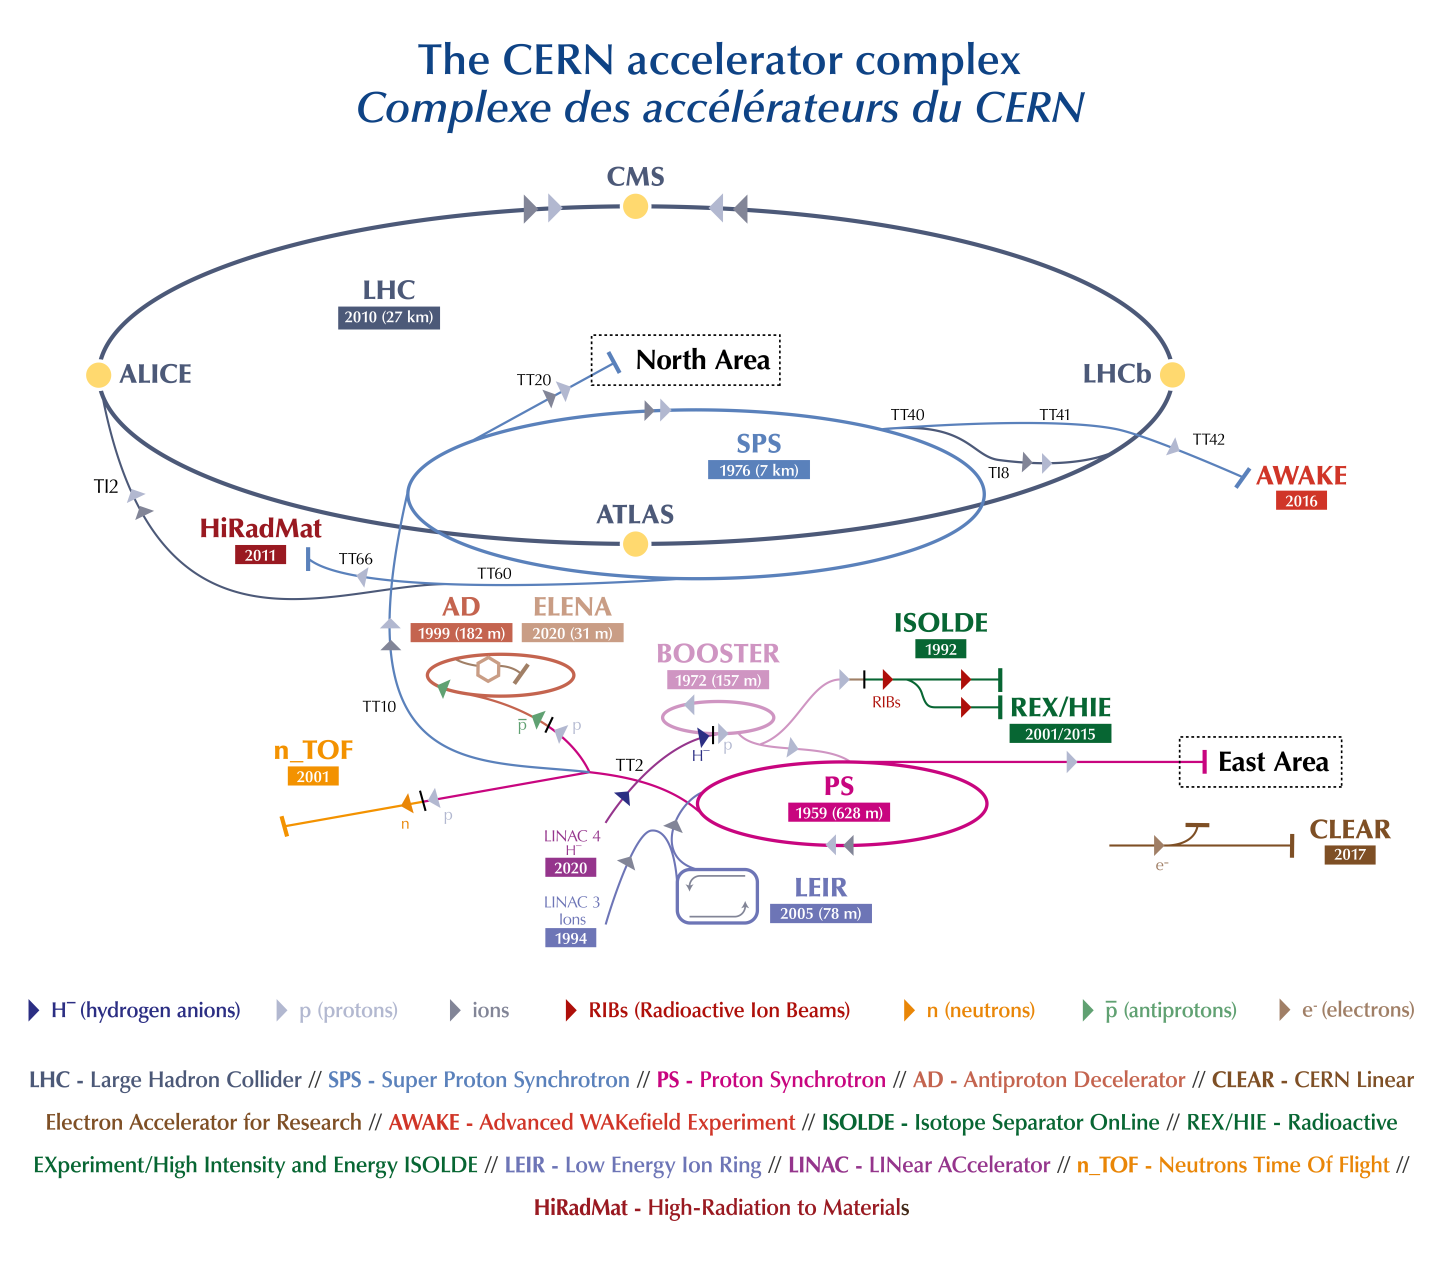
\includegraphics[width=0.75\textwidth]{figuresEXP/LHC1.png}
  \end{center}
  \caption{
CERN加速器系统的结构。首先质子会被注入到直线加速器\textsc{Linac2}当中,
然后将它们注入到环形加速器\textsc{Booster}当中,随后,会将它们送入环形加速器\textsc{Ps}当中,
接着,在经过环形加速器\textsc{Sps}加速之后,最后进入LHC大环,此时质子能量可以达到7TeV。
  }
    \label{fig:LHC1}
\end{figure}


在质子束流由环形加速器\textsc{Sps}向LHC大环转移的过程中,束流会被分成两个单独的束流,分别沿着相反的方向注入到LHC大环当中,然后进行碰撞。
束流中的质子束是以非连续的形式组合在一起的,每个质子束大约含有$10^{11}$个质子。
而单个束流最多包含2808个质子束,质子束与质子束之间碰撞的时间间隔为25ns,碰撞频率高达40MHz。
根据设计,束流能达到最高7TeV的能量,对应的质心系能量为$\sqrt{s}$=14TeV。
瞬时亮度(Instantaneous luminosity)能达到$\mathcal{L}=10^34 cm^{-2}s^{-1}$~\cite{Evans:2008zzb}。

LHC于2008年9月正式开始运行,但是在开始调试阶段,由于其中两个磁铁之间的电气故障,对整个机器造成了严重的损坏。
经过一段时间的修复之后,2010年3月,$Run\_1$计划正式启动,LHC首次以7TeV的质心系能量实现了质子-质子对撞,
这样一直持续到2011年底,对撞数据总积分亮度(Integrated luminosity)达到了5.5$fb^{-1}$。
在2012年,束流能量提升到了4TeV,在质心系能量为8TeV的条件下成功运行了一年,这一年里数据总积分亮度大约为23$fb^{-1}$。
到此,$Run\_1$计划顺利结束。
LHC经过两年的设备维修和加速器升级之后,
$Run\_2$计划于2015年3月正式开始,此时质子束流的能量达到了6.5TeV,从而质心系能量高达13TeV。
仅在2015年底因为重离子碰撞实验的进行有短暂的停机之外,对撞数据的采集一直持续到2018年底,这也标志着$Run\_2$计划的结束。
如图~\ref{fig:LHC2}所示,从2015年到2018年,LHC实现了数据总积分亮度为156$fb^{-1}$的质子-质子对撞~\cite{ATLASWEB1}。

\begin{figure}
  \begin{center}
    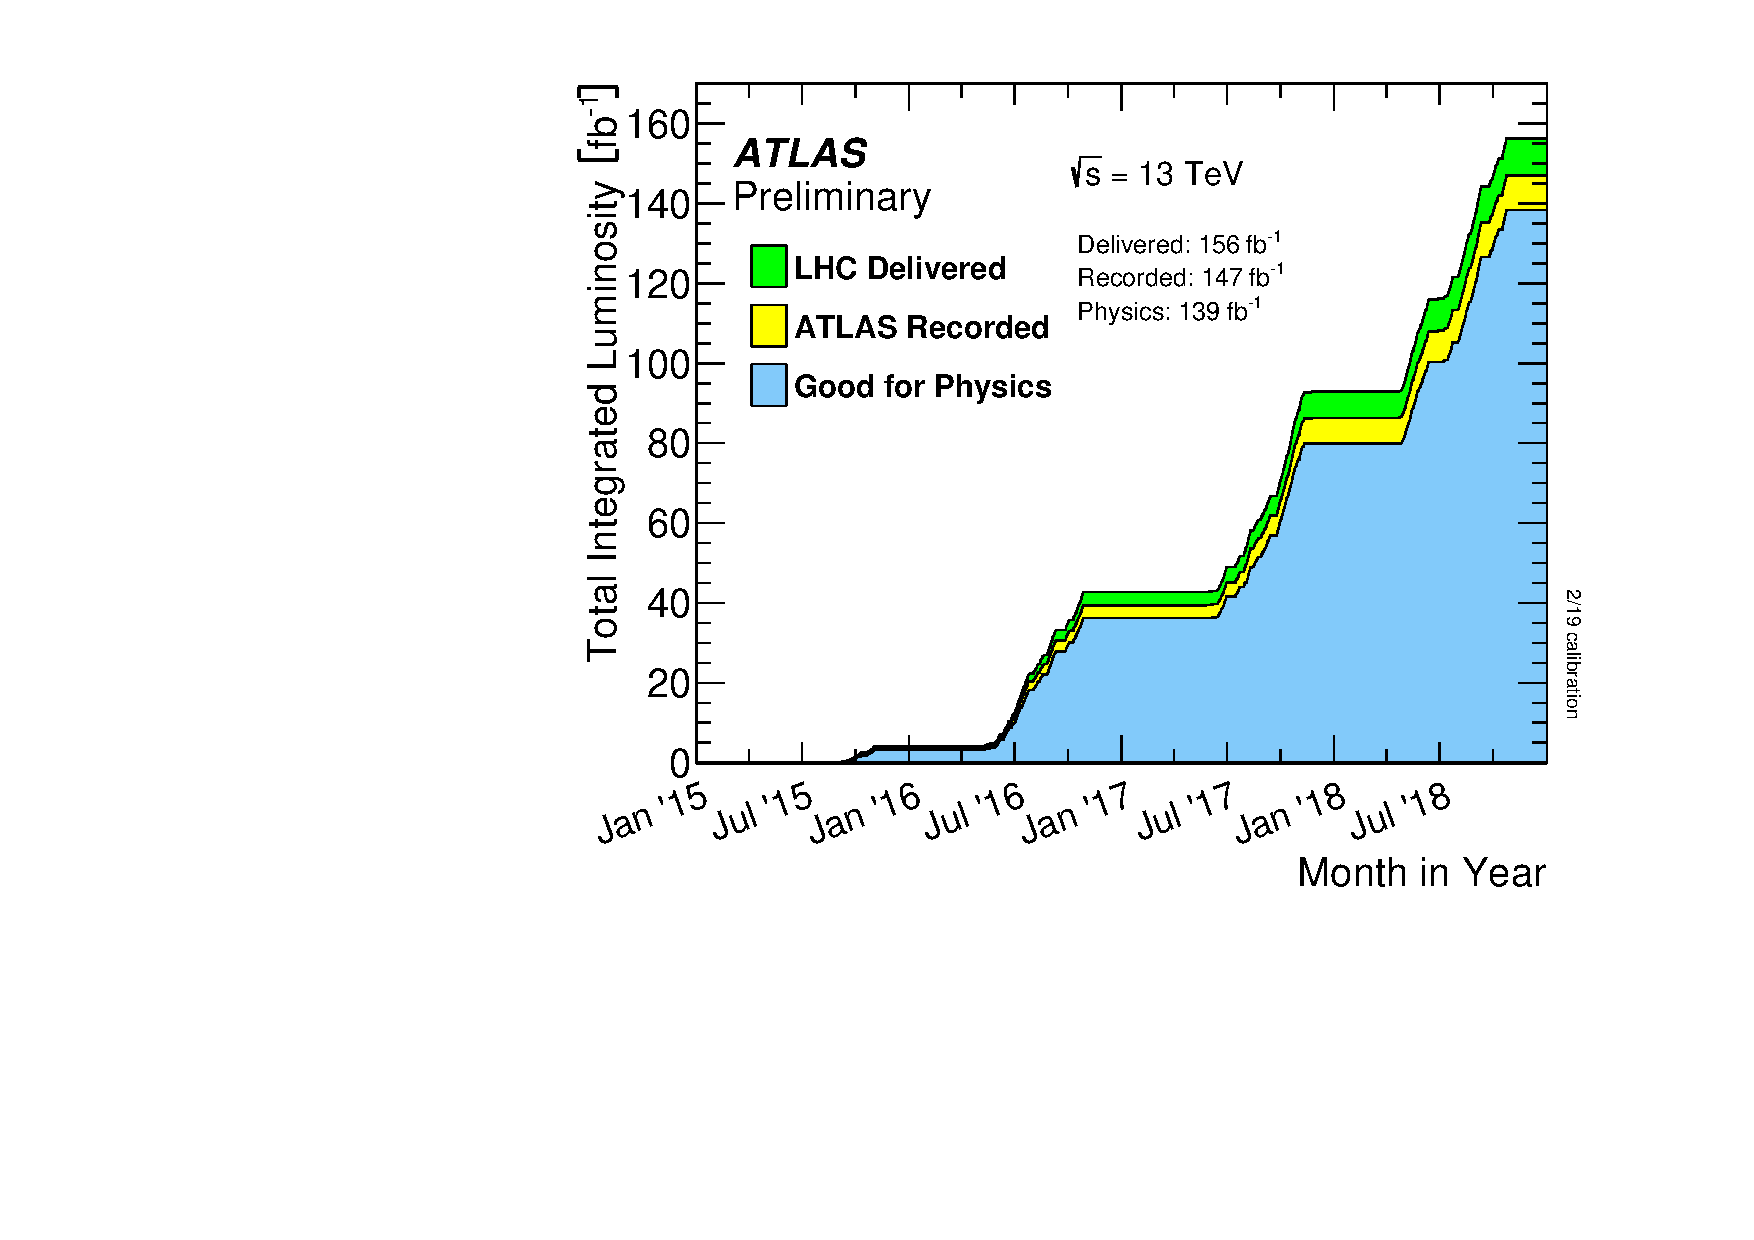
\includegraphics[width=0.75\textwidth]{figuresEXP/LHC2.pdf}
  \end{center}
  \caption{
  $Run\_2$计划期间LHC上质子-质子对撞数据的总积分亮度。
  到2018年底,LHC实现的数据总积分亮度为156$fb^{-1}$,
  ATLAS探测器所收集的数据总积分亮度为147$fb^{-1}$,
  在设备运转正常和数据采集稳定的情况下可用于实际物理分析的数据总积分亮度为139$fb^{-1}$。
  }
    \label{fig:LHC2}
\end{figure}

高能量和高密度的质子束流对撞为基本粒子的研究提供了可能。
LHC上有四个束流碰撞点,每个碰撞点都有一个实验,
共四个实验分别用于高能物理领域不同方面的研究:
%LHC上对应于束流四个碰撞点的四个实验分别用于研究基本粒子领域的不同方面:
其中ATLAS~\cite{PERF-2007-01}和CMS~\cite{CMS}是两个大型的通用型探测器,
用于标准模型的精确测量和寻找超出标准模型的新物理;
LHCb(Large Hadron Collider beauty)~\cite{LHCb}是一个用于研究B介子物理的正向探测器;
ALICE(A Large Ion Collider Experiment)~\cite{ALICE}是一个用于研究重离子碰撞的探测器。
%的研究着重于重离子碰撞。
其中ATLAS探测器在$Run\_2$计划期间所收集的数据总积分亮度为147$fb^{-1}$,
在设备运转正常和数据采集稳定的情况下可用于实际物理分析的数据总积分亮度为139$fb^{-1}$。
束流相交时非常高的质子-质子碰撞频率给探测器带来了极大的挑战,
同时也因为高密度的质子束流使得两个单独的质子束相交时能够产生多次碰撞(堆积事例,pileup)~\cite{PileUp},让探测器中事例的重建也非常具有挑战性。
图~\ref{fig:LHC3}的是ATLAS实验在$Run\_2$计划期间记录的质子束相交时发生碰撞的平均次数的简况图~\cite{ATLASWEB1}。
总体来说,ATLAS实验在$Run\_2$计划期间收集的质子束相交时发生碰撞的平均次数为$\langle\mu\rangle=33.7$。
论文后面的物理分析所用到的数据便是由\textsc{ATLAS}实验在$Run\_2$计划期间收集的,下一部分将对ATLAS实验做更加详细的介绍。

\begin{figure}
  \begin{center}
    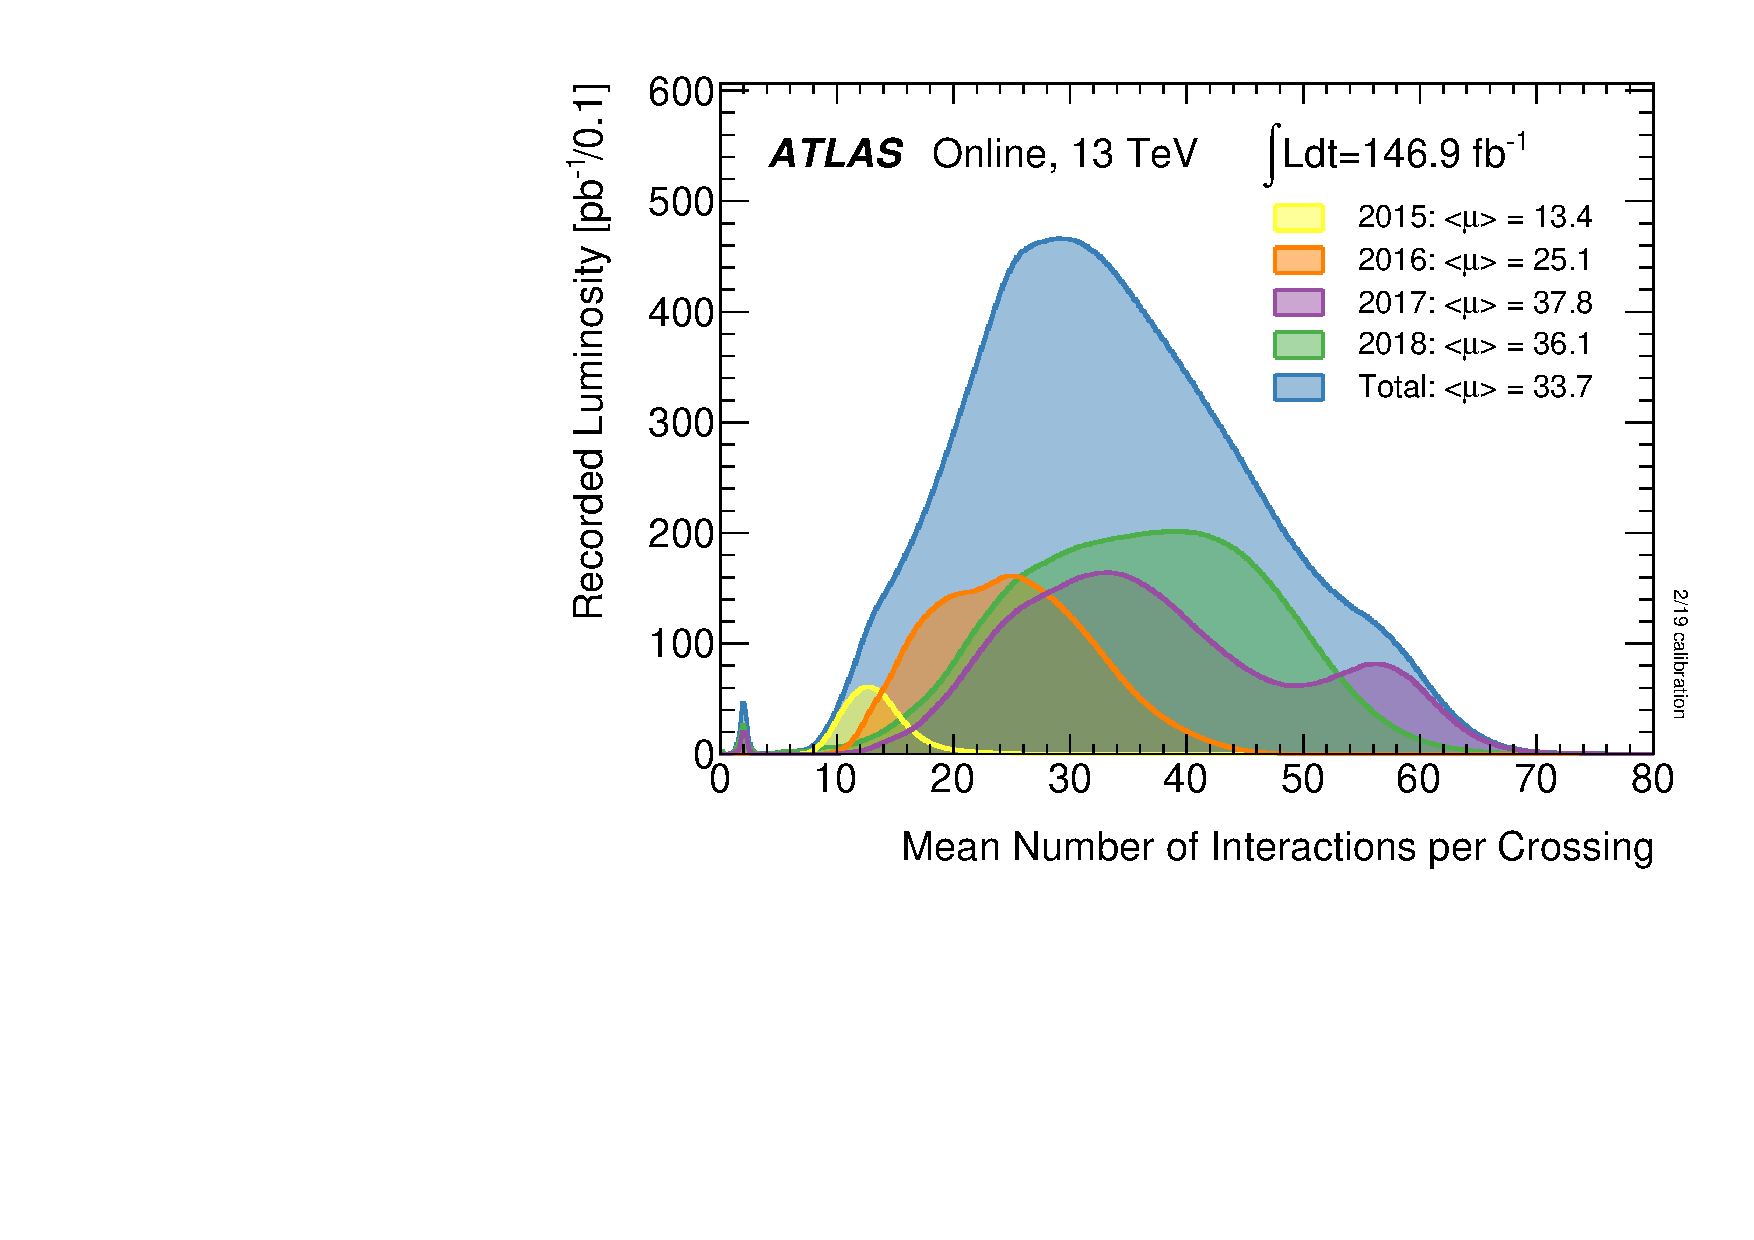
\includegraphics[width=0.75\textwidth]{figuresEXP/LHC3.pdf}
  \end{center}
  \caption{
  $Run\_2$计划期间\textsc{ATLAS}实验记录的质子束相交时发生碰撞的平均次数。图示为四年中堆积事例的概况,
  在2017年有个两个峰值是因为年中LHC操作方案的调整。
    }
    \label{fig:LHC3}
\end{figure}


\section{ATLAS探测器}
\label{sec:ATLAS}

\textsc{ATLAS}(A Toroidal LHC ApparatuS)~\cite{PERF-2007-01,ATLASPERF1,ATLASPERF2}探测器是一个用于粒子物理研究的通用型探测器,通过它能观察到质子-质子对撞过程产生的所有衰变产物。它是有史以来人类建造的体积最大的粒子探测器,如图~\ref{fig:ATLAS1}所示是探测器的一张截面图,它关于碰撞点前后对称,其圆柱形桶身几乎覆盖了整个$4\pi$立体角。而且整个探测器长44m,宽25m,重达7000吨,位于地下约100m处的LHC其中一个质子-质子对撞点。

\begin{figure}
  \begin{center}
    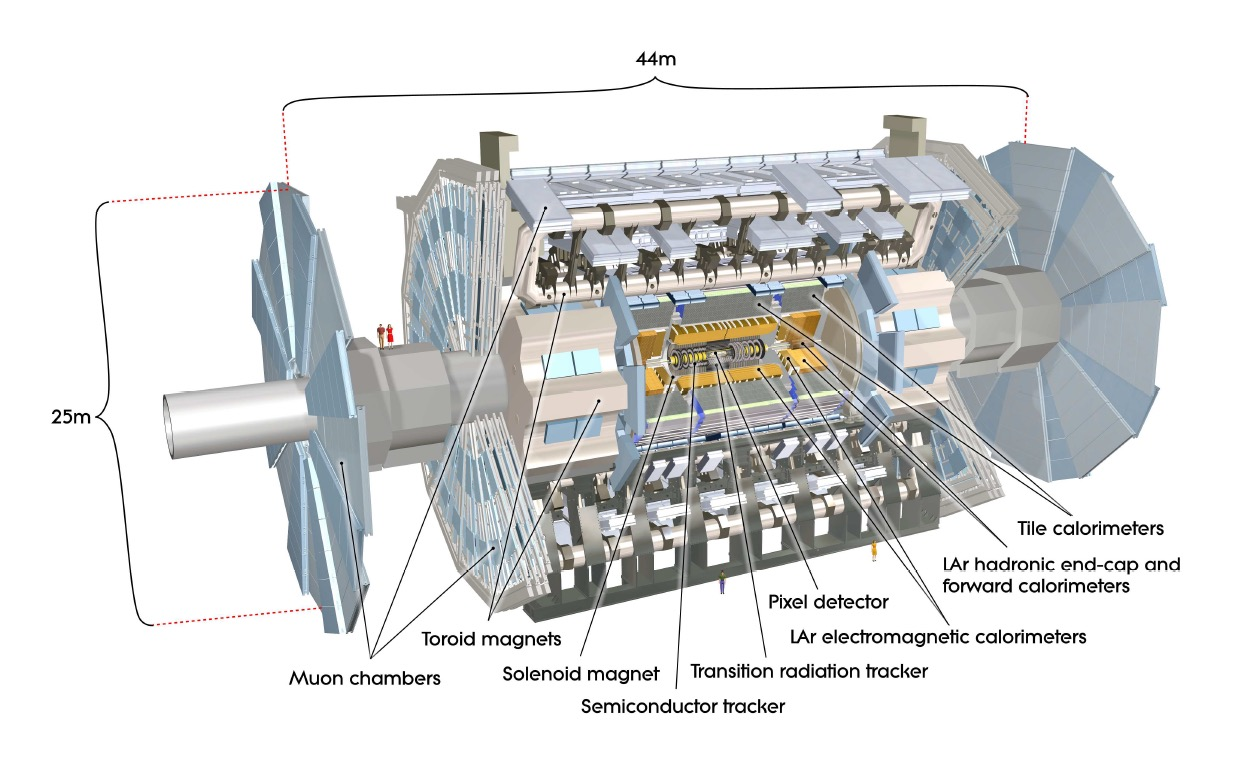
\includegraphics[width=0.75\textwidth]{figuresEXP/ATLAS1.jpg}
  \end{center}
  \caption{
整个\textsc{ATLAS}探测器的截面图和它的子结构。
  }
    \label{fig:ATLAS1}
\end{figure}

LHC中高亮度和高能量的质子束流对撞使得探索TeV量级的物理学成为可能,\textsc{ATLAS}的设计初衷主要基于以下几个目标:
希格斯玻色子的寻找及其基本性质的测量;
量子色动力学、电弱相互作用、味物理等标准模型的精确测量;
超出标准模型的新物理的寻找,比如暗物质、新的重玻色子等;
t夸克性质的精确测量,比如质量、耦合常数和自旋等;
寻找超对称等标准模型的延拓理论。

为了能处理约高达$6\times10^8s^{-1}$的质子-质子非弹性碰撞事例产生率,\textsc{ATLAS}探测器的设计需要满足几个条件:
抗辐照且高速的电子设备和传感器元件、高粒度的探测器材料,用于处理高通量的粒子和减小重叠事例带来的影响;
覆盖几乎整个方位角的高接收度;
能精确追踪带电粒子,比如高的动量分辨率,径迹重建率和第二顶点重建率等;
精确的电磁量能技术和强子量能技术,用于电子、光子和喷注等能量测量;
精确的识别和高的动量分辨率。
为此,\textsc{ATLAS}采用层叠式设计,从里到外由不同的子探测器组成,均匀覆盖在束流管和对撞点周围,
它们依次是内部探测器(the Inner Detector, ID)~\cite{ATLASINNER}、电磁量能器(the Electromagnetic Calorimeter)、
强子量能器(the Hadronic Calorimeter)、前端量能器(the Forward Calorimeter)~\cite{ATLASLACA,ATLASTCA}、
$\mu$子谱仪(the Muon Spectrometer)~\cite{ATLASMUSPEC}和亮度探测器(the Luminosity Detectors)~\cite{ATLASLUMID}。
其中,内部探测器处于一个平行于束流轴的强度为2T的恒定磁场中,它可以测量带电粒子的运动方向、动量和电荷,也用来重建碰撞顶点。
量能器用来吸收光子、电子和强子并测量它们的能量,它能吸收除$\mu$子和中微子之外的所有已知粒子。
$\mu$子谱仪位于探测器的最外面,它被包围在一个恒定的强磁场中,磁场由超导磁铁产生,从而它能以很高的精度测量$\mu$子的轨迹和动量。
三个亮度探测器位于\textsc{ATLAS}探测器前端
%依次是切伦科夫亮度探测器(the Luminosity measurement using Cerenkov Integrating Detector, LUCID)、零能探测器(the Zero-Degree Calorimeter, ZDC)和绝对亮度探测器(the Absolute Luminosity For ATLAS, ALFA)
,用来测量亮度。
表~\ref{tab:ATLASTab1}展示的是\textsc{ATLAS}探测器的子探测器的主要性能目标。

\begin{table}[htbp]
      \caption{\textsc{ATLAS}探测器的子探测器的主要性能目标。}
      \label{tab:ATLASTab1}
      \centering
      \begin{adjustbox}{width=\columnwidth,center}
      \begin{tabular}{|c|c|c|c|}
         \hline
         Detector component & Required resolution & \thead{$\eta$ coverage \\ (Measurements)} & \thead{$\eta$ coverage \\ (Trigger) } \\
        \hline
         Tracking & $\sigma_{p_{T}}/p_{T}=0.05\%/\sqrt{p_{T}}\oplus 0.01\%$  & $\pm2.5$ &  \\
        \hline
         EM calorimetry & $\sigma_{E}/E=10\%/\sqrt{E}\oplus 0.7\%$ & $\pm3.2$ & $\pm2.5$  \\
         \hline
         \thead{Hadronic calorimetry (jets) barrrel \\ and end-cap forward} & $\thead{\sigma_{E}/E=50\%/\sqrt{E}\oplus 3\% \\ \sigma_{E}/E=100\%/\sqrt{E}\oplus 10\%}$ & $\thead{\pm3.2 \\ 3.1<|\eta|<4.9}$ & $\thead{\pm3.2 \\ 3.1<|\eta|<4.9}$  \\
         \hline
         Muon spectrometer & $\sigma_{p_{T}}/p_{T}=10\% \quad at \quad p_{T}=1TeV$ & $\pm2.7$ & $\pm2.4$  \\
         \hline
      \end{tabular}
      \end{adjustbox}
\end{table}

粒子的重建是根据粒子与探测器材料的相互作用实现的,如图~\ref{fig:ATLAS2}所示,是\textsc{ATLAS}探测器中鉴别和重建粒子的过程简图~\cite{ATLASTool}。
带电粒子在ATLAS最里面的内部探测器中会留下电离信息,以此来重建它的径迹,但是电中性的粒子比如说中微子不会,其中的磁场会使带电粒子发生偏转,由此来重建动量和电荷。
除中微子之外,所有粒子都会在电磁量能器和强子量能器中沉积一部分或者全部的能量,电磁量能器主要用于沉积光子和电子能量,强子量能器
主要用于沉积强子能量。
电子、光子、质子和中子会在量能器中产生一团簇射并最终停留在里面,而$\mu$子会穿过前面的内部探测器和量能器,在量能器中沉积一小部分能量之后,最终停在$\mu$子谱仪当中。
中微子因为其独特的性质不能被\textsc{ATLAS}探测器探测到,重建过程中通过事例中动量守恒来推断它们的存在。
后续将对\textsc{ATLAS}探测器的子探测器和粒子重建做更加详细的描述。

\begin{figure}
  \begin{center}
    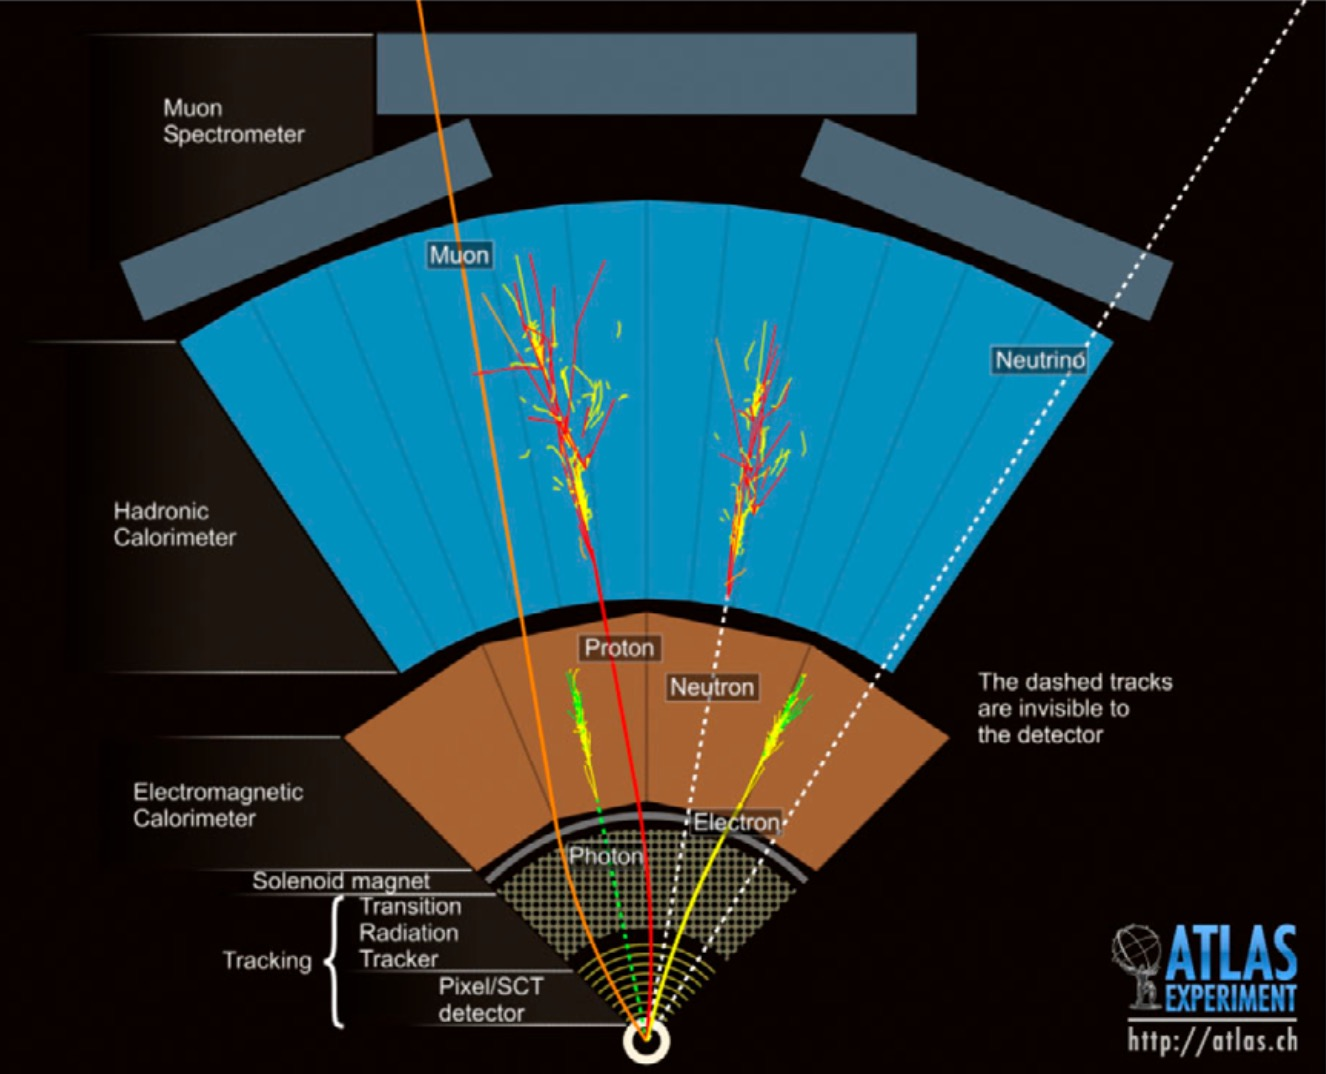
\includegraphics[width=0.75\textwidth]{figuresEXP/ATLAS2.jpg}
  \end{center}
  \caption{
 不同粒子如何和\textsc{ATLAS}探测器中子探测器相互作用的图示。
  }
    \label{fig:ATLAS2}
\end{figure}

\subsection{坐标系}
\label{sec:ATLASCS}

在\textsc{ATLAS}实验所使用的坐标系中,原点位于标准的质子-质子对撞点,$z$轴指向束流方向,$x$轴指向LHC大环中心,$y$轴垂直于$x$-$z$平面向上。如图~\ref{fig:ATLAS3}所示为坐标系简图,$x$-$y$平面为束流的横截面。

\begin{figure}
  \begin{center}
    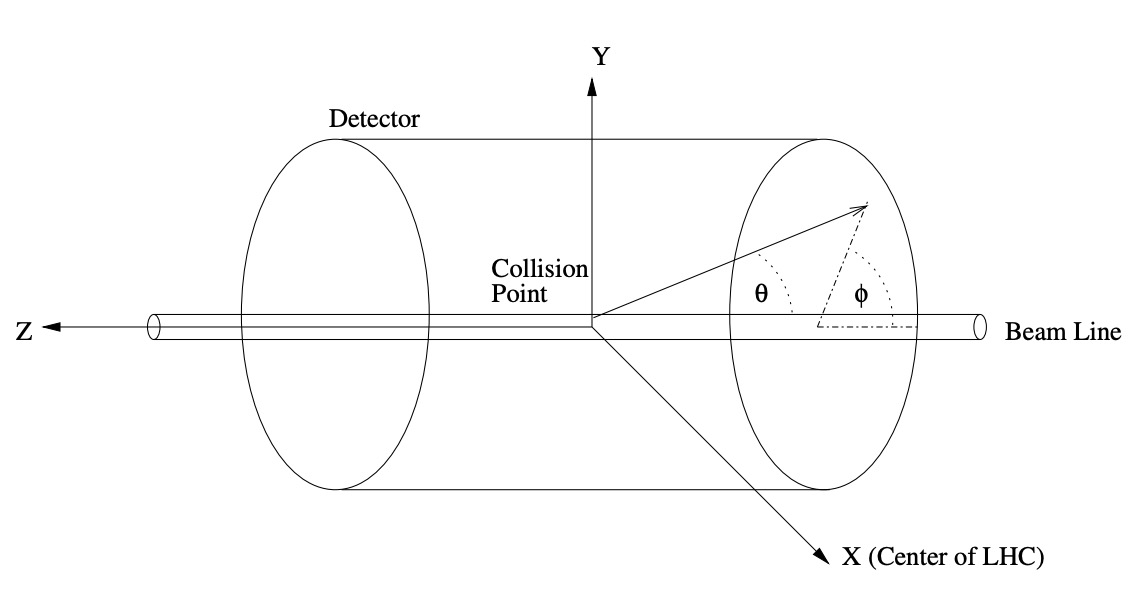
\includegraphics[width=0.75\textwidth]{figuresEXP/ATLAS3.jpg}
  \end{center}
  \caption{
 \textsc{ATLAS}实验所使用的坐标系。
  }
    \label{fig:ATLAS3}
\end{figure}

根据探测器的对称性,也可以使用柱坐标系$(R,\phi,\theta)$,其中$R=\sqrt{x^2+y^2}$,$\theta$是与束流轴所成的夹角,$\phi$是绕束流轴的方位角。这里引入快度$y$,其定义为:
\begin{equation} 
\label{eq:ydef}
y=\frac{1}{2}ln\left( \frac{E+p_{z}}{E-p_{z}} \right)
\end{equation}
其中$E$和$p_{z}$分别是粒子的能量和动量沿轴方向的分量。可以证明$\Delta y$在沿$z$轴方向的洛伦兹变换下是不变的。
如果粒子的质量相对于粒子的能量可以忽略不计,则快度$y$可以近似成赝快度$\eta$:
\begin{equation} 
\label{eq:etadef}
\eta=-ln\left(\tan\frac{\theta}{2} \right)
\end{equation}
其中$\theta$为极角,$\eta$是描述粒子相对于束流轴所成夹角的常用空间坐标,
图~\ref{fig:ATLAS4}在坐标平面上展示了不同的赝快度$\eta$所对应的极角值$\theta$。
横动量$p_{T}=\sqrt{p_x^2+p_y^2}$和横能量$E_{T}=E\sin\theta$分别定义为粒子沿$x$-$y$平面的动量和能量。
$\Delta R$定义为粒子在$\eta$-$\phi$空间的距离:
\begin{equation} 
\label{eq:DRdef}
\Delta R=\sqrt{\Delta\eta^2+\Delta\phi^2}
\end{equation}
其中$\Delta\eta$和$\Delta\phi$分别为粒子的赝快度之差和方位角之差。

\begin{figure}
  \begin{center}
    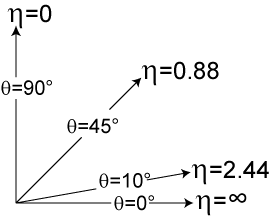
\includegraphics[width=0.5\textwidth]{figuresEXP/ATLAS4.png}
  \end{center}
  \caption{
赝快度$\eta$和所对应的极角$\theta$值。
  }
    \label{fig:ATLAS4}
\end{figure}


\subsection{磁系统}
\label{sec:ATLASMS}

为了精确地重建带电粒子径迹及测量带电粒子动量和电荷,探测器需要一个非常强的磁场。当一个动量为$p$、带电量为$q$的粒子垂直进入一个磁场强度为$B$的磁场时,受洛伦兹力作用,粒子运动的曲率半径$\rho$为:
\begin{equation} 
\label{eq:rhodef}
\rho=\frac{p}{q\cdot B}
\end{equation}
因此,为了确定带电粒子的动量,需要测量其通过磁场中探测器时轨迹的曲率半径。
如图~\ref{fig:ATLAS5}所示,\textsc{ATLAS}探测器中包含两个由以下四个大型的超导磁体提供的独立磁系统~\cite{ATLASMS}:
位于内部探测器和电磁量能器之间并与束流轴对齐的中心螺线管(Central Solenoid, CS),
它的直径为2.4m,长5.3m,能为内部探测器提供一个强度为2T的轴向磁场,同时能最小化桶部电磁量能器前的辐射厚度;
25m长的桶部环形磁体(Barrel Toroid, BT)和两组5m长的端盖环形磁体(End-Cap Toroids, ECT),
它们能为$\mu$子谱仪提供一个与$\mu$子轨迹接近垂直的强度为4T的环形磁场。
整个磁系统置于在温度为4.8K的液氦中。

\begin{figure}
  \begin{center}
    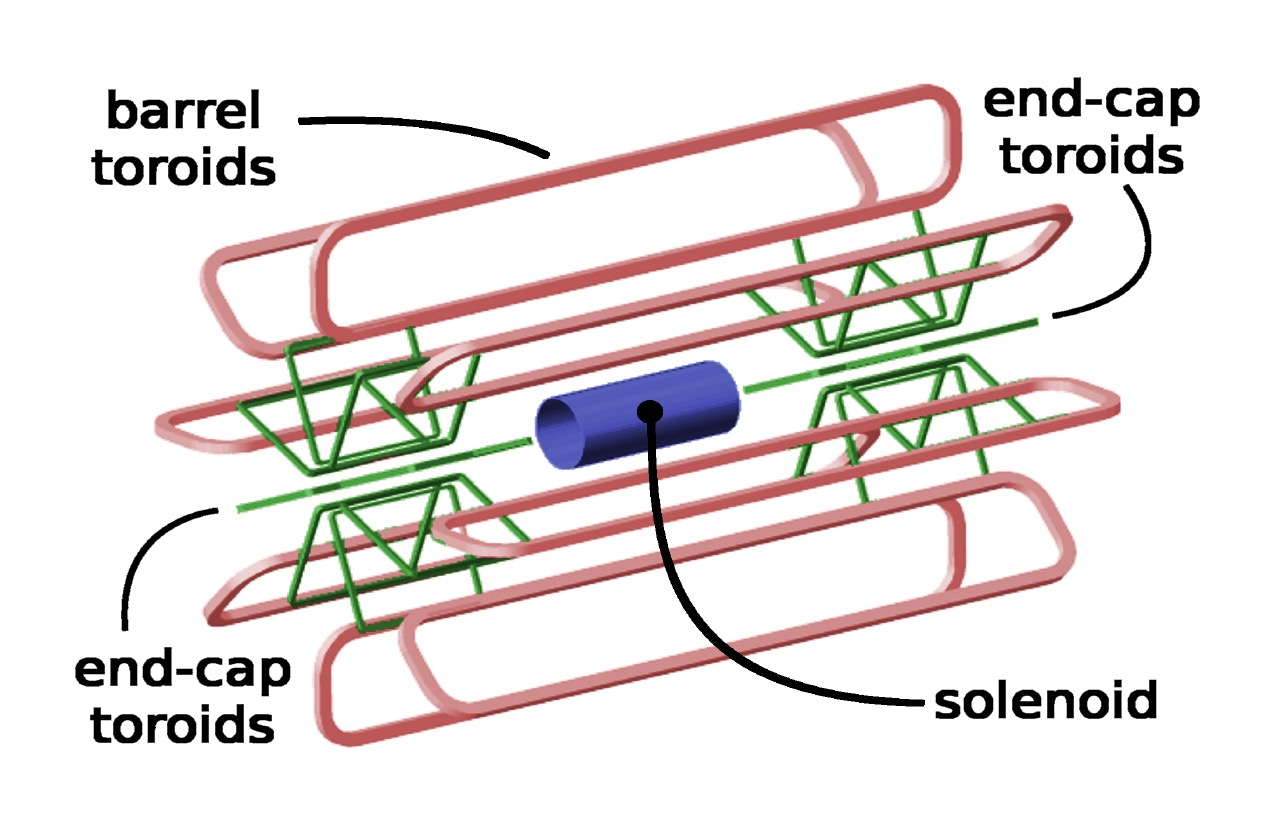
\includegraphics[width=0.75\textwidth]{figuresEXP/ATLAS5.jpg}
  \end{center}
  \caption{
 \textsc{ATLAS}探测器中磁系统的布局。
  }
    \label{fig:ATLAS5}
\end{figure}

\subsection{内部探测器}
\label{sec:ATLASID}

如图~\ref{fig:ATLAS6}所示,是ATLAS内部探测器(the Inner Detector, ID)的截面图,它是由桶部和端盖上同心的多层探测材料组成,离对撞点最近,主要用于高精度的重建带电粒子的动量、径迹和事例的主顶点、第二顶点等信息,覆盖了$|\eta|<2.5$的范围。
它长6.2m,端盖半径为1.1.m,并处于一个强度为2T的螺线管磁场中。

\begin{figure}
  \begin{center}
    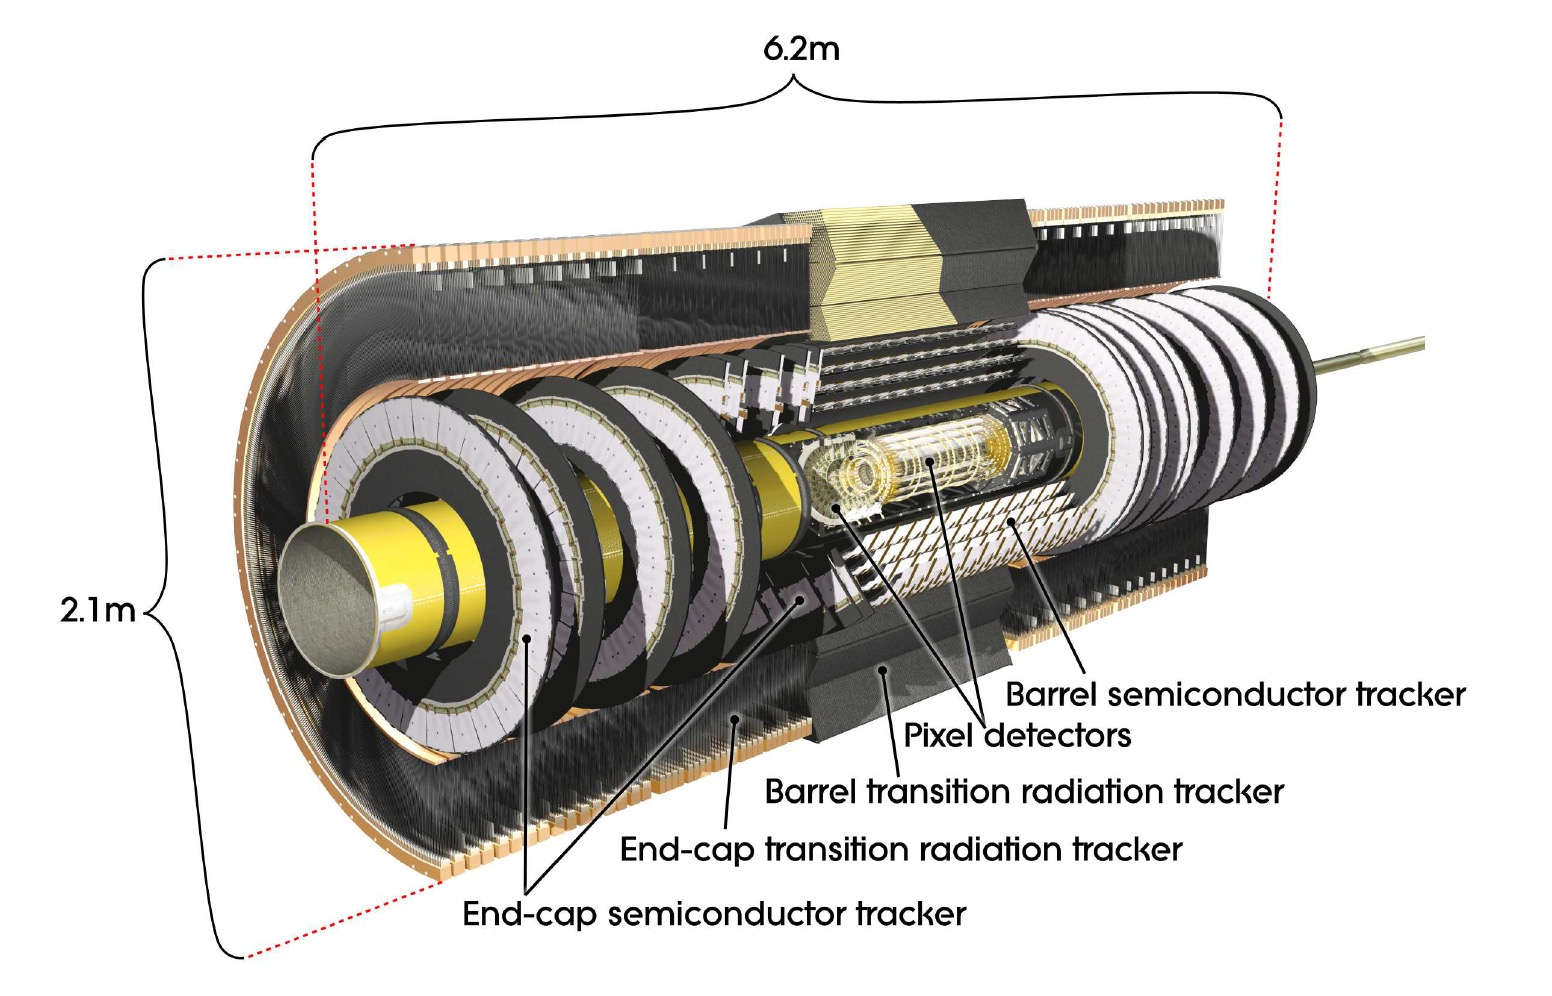
\includegraphics[width=0.75\textwidth]{figuresEXP/ATLAS6.jpg}
  \end{center}
  \caption{
 \textsc{ATLAS}内部探测器的截面图和它的子结构。
  }
    \label{fig:ATLAS6}
\end{figure}

为了实现高精度的径迹和顶点重建,它是由四个高粒度且互补的子探测器组成,如图~\ref{fig:ATLAS7},从最里层到最外层,依次是嵌入式B层探测器、像素探测器、半导体径迹探测器和跃迁辐射径迹探测器。

\begin{figure}
  \begin{center}
    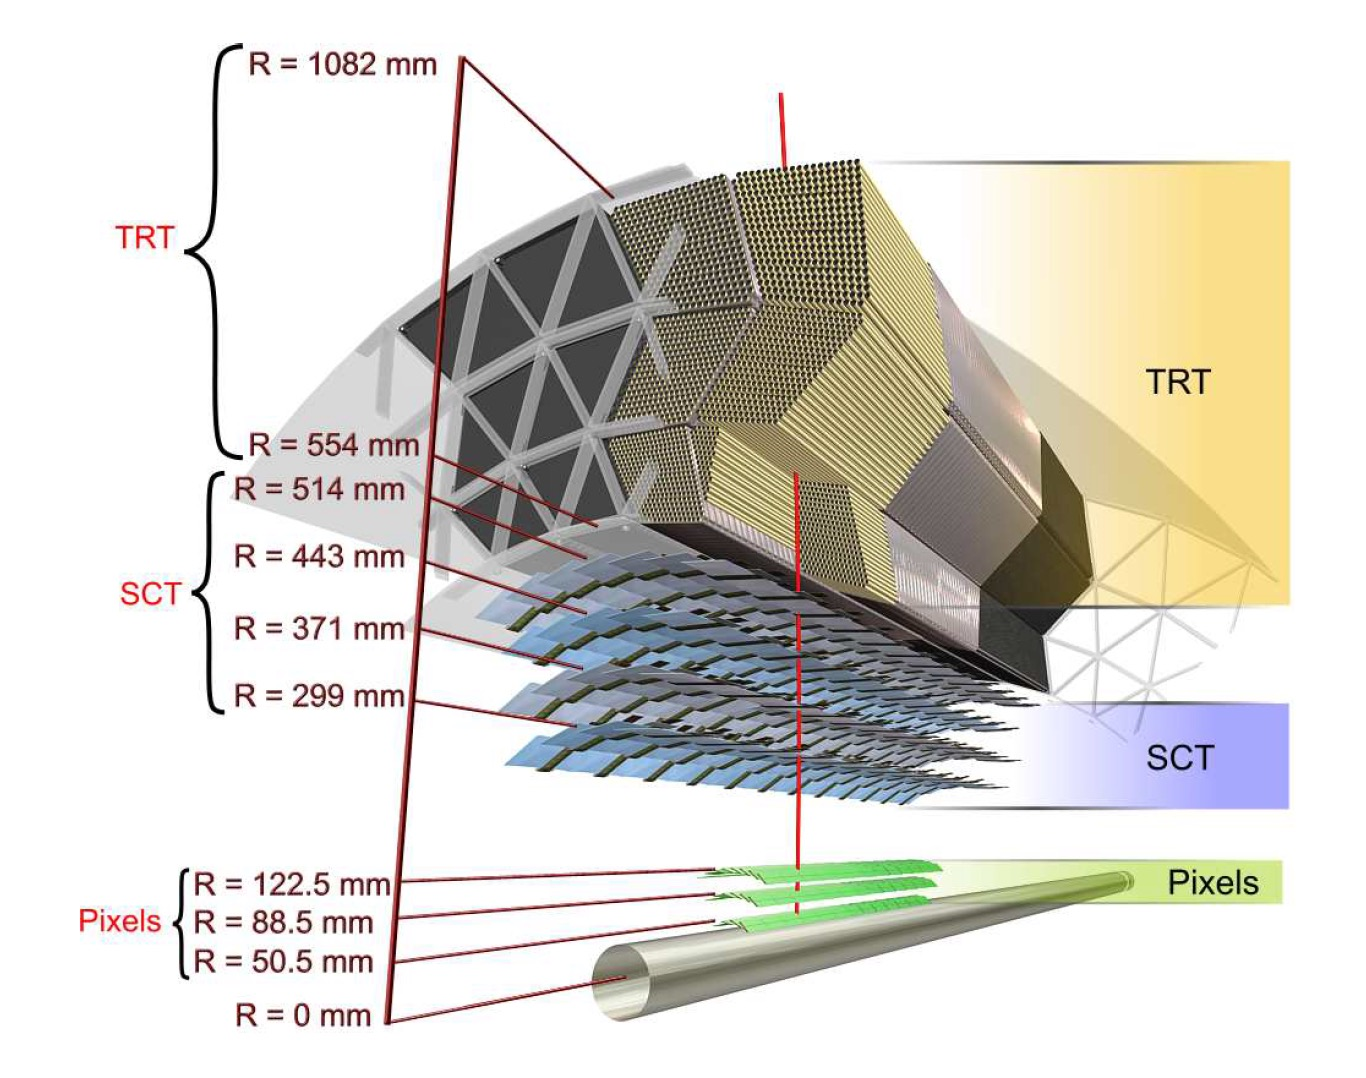
\includegraphics[width=0.75\textwidth]{figuresEXP/ATLAS7.jpg}
  \end{center}
  \caption{
 \textsc{ATLAS}内部探测器的桶部子探测器的截面简图。灰色的小圆柱是LHC的束流管。嵌入式B层探测器(LBL)是在$Run\_2$计划期间安装的。
  }
    \label{fig:ATLAS7}
\end{figure}

嵌入式B层探测器(the Insertable B-Layer, IBL)~\cite{ATLASIBL}是内部探测器中离束流管最近的一个子探测器。
$Run\_2$计划面临的主要问题之一是总积分亮度的显著增加会给内部探测器带来很大的辐照损伤,
进而会导致内部探测器的径迹重建效率下降,尤其是b-jet的重建效率。
嵌入式B层探测器正是在这样一个背景下加入到ATLAS的内部探测器中的,它是在$Run\_2$计划执行之前安装的,
呈柱状,半径33.2mm,长3.5m,位于铍制束流管和像素探测器的第一层之间。
为了处理束流的高亮度,它不仅抗辐照,而且其中的每个像素传感器单元的尺寸很小,仅有50$\mu m$×250$\mu m$($R$-$\phi\times z$),固有精度是8$\mu m$($R$-$\phi$)和40$\mu m$($z$),覆盖了整个$0\le\phi<2\pi$的范围。
嵌入式B层探测器对测量精确的提升非常显著,如图~\ref{fig:ATLAS8},是碰撞参数$d_0$的分辨率变化曲线的前后对比图,
其中碰撞参数$d_0$定义为$x$-$y$平面上径迹中离$z$轴最近的点与$z$轴之间的距离,它是影响b-jet标定性能的关键参数。
除了碰撞参数的分辨率,嵌入式B层探测器对顶点重建的效率和b-jet标定性能~\cite{IBLBP}也有明显的提升。
这些提升主要是因为嵌入式B层探测器相对于像素探测器更靠近束流并能分辨更小的尺度。

\begin{figure}
  \begin{center}
    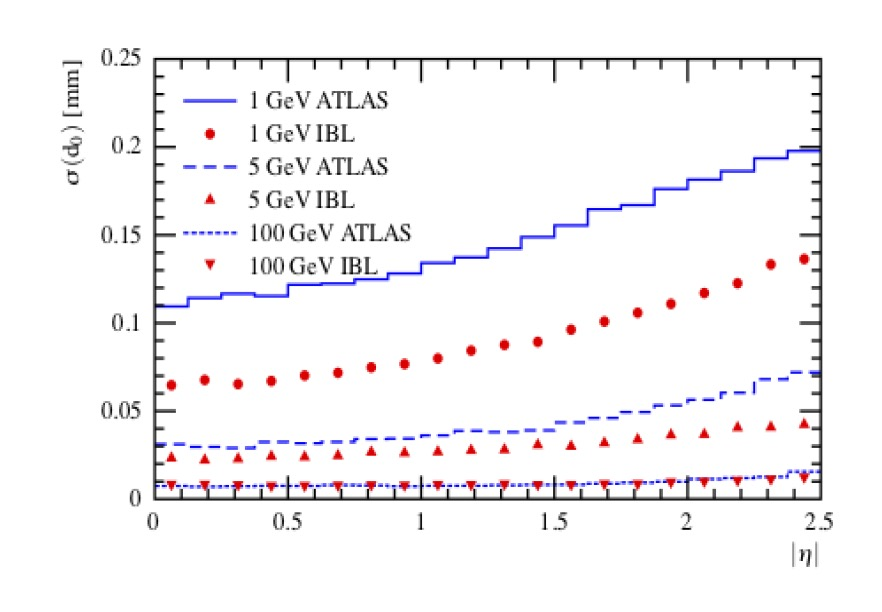
\includegraphics[width=0.75\textwidth]{figuresEXP/ATLAS8.jpg}
  \end{center}
  \caption{
 内部探测器中未安装和安装嵌入式B层探测器的情况下,单$\mu$子碰撞参数的分辨率随着赝快度$\eta$的变化关系。
  }
    \label{fig:ATLAS8}
\end{figure}

像素探测器(the Pixel Detector, PD)为对撞点附近的模式识别提供关键的径迹信息。
如图~\ref{fig:ATLAS9}所示,它是由三个分别位于以束流轴为中心的半径为51mm、89mm和123mm处的桶层结构和左右两边两个端盖结构组成,其中每个端盖具有三个圆盘层,分别位于$|z|$=495mm、$|z|$=580mm和$|z|$=650mm处。
它能为$|\eta|<2.5$、$0\le\phi<2\pi$范围内的径迹提供三个或者更多个精确测量点。
端盖和桶层结构中硅像素传感器~\cite{PDSS}的尺寸都是50$\mu m$×400$\mu m$($R$-$\phi\times z$),
固有精度都为10$\mu m$($R$-$\phi$)和115$\mu m$($z$)。
整个像素探测器总共有大约80万个读出信道。
$R$-$\phi$平面和沿束流轴方向的高分辨率对于精确重建动量、径迹、主顶点和第二顶点来说起着至关重要的作用。

\begin{figure}
  \begin{center}
    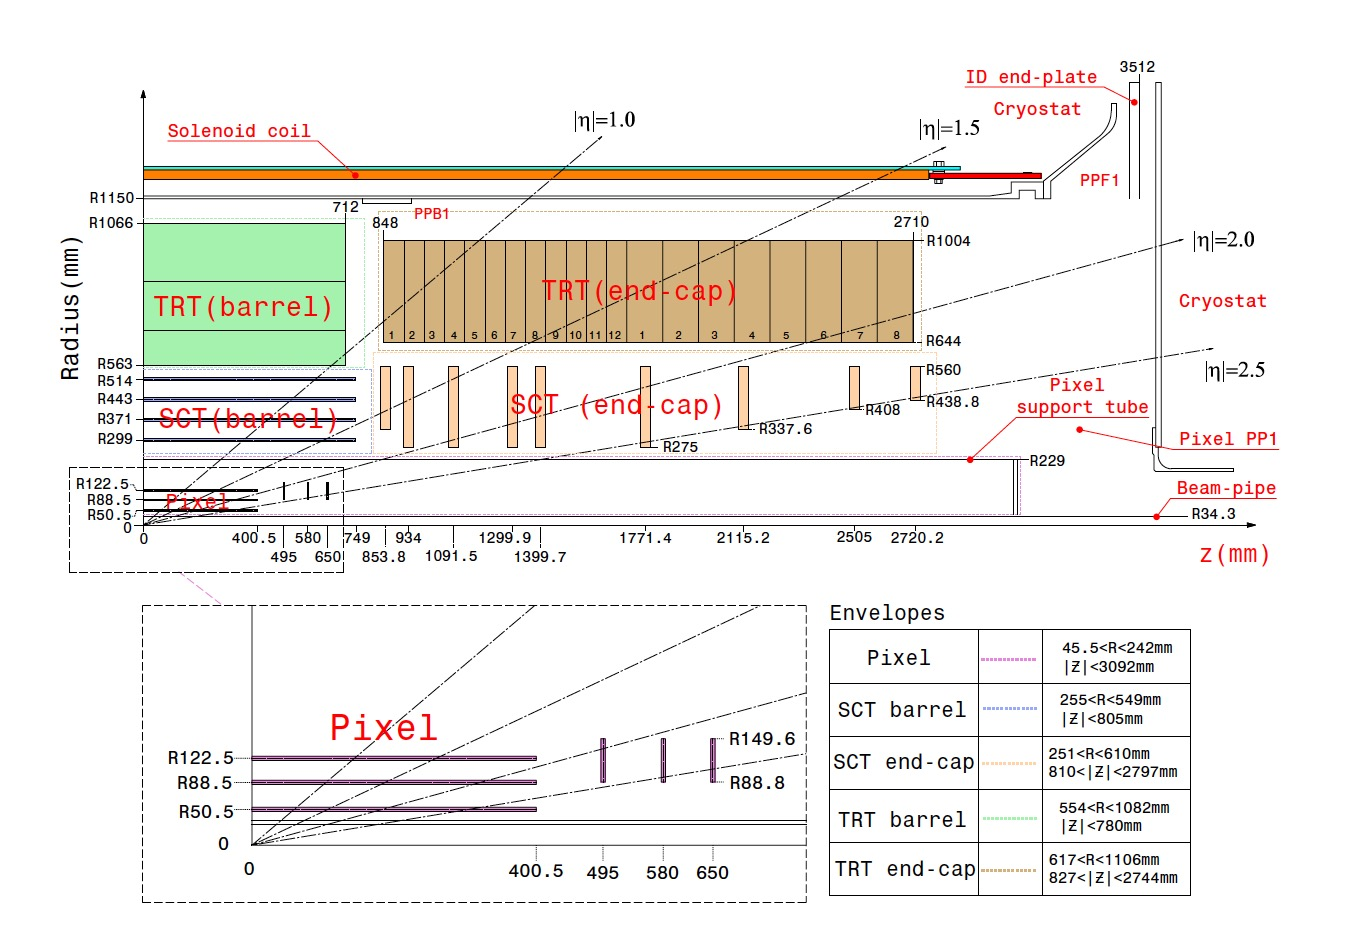
\includegraphics[width=0.75\textwidth]{figuresEXP/ATLAS9.jpg}
  \end{center}
  \caption{
ATLAS内部探测器沿$R$-$z$平面的截面图。图中展示了其中各个子探测器的结构和尺寸等,左下部分是像素探测器的放大图。
  }
    \label{fig:ATLAS9}
\end{figure}

半导体径迹探测器(the SemiConductor Tracker, SCT)位于内部探测器的中间位置,采用了与像素探测器相同的半导体技术,
并使用尺寸为120mm$\times$60mm($\phi\times z$)的硅微条~\cite{SCTSS}作为测量元件,同样覆盖了$|\eta|<2.5$、$0\le\phi<2\pi$的范围。
如图~\ref{fig:ATLAS9}所示,它是由四个桶层结构(299mm<$R$<514mm)和左右两边两个各含九个圆盘层的端盖结构(850mm<$z$<2730mm)组成,
其中四个分别由两层传感器构成的桶层结构位于以束流轴为中心的半径为30cm、37cm、44cm和51cm处。
端盖和桶层结构的固有精度都是17$\mu m$($R$-$\phi$)和580$\mu m$($z$),
整个半导体径迹探测器共有6.3万个读出信道,
能在$R$坐标和$z$坐标为每条径迹提供四个额外的空间测量点。
它的测量精度略低于像素探测器的测量精度,但是在重建动量、径迹和顶点方面仍发挥着重要作用。

跃迁辐射径迹探测器(the Transition Radiation Tracker, TRT)位于内部探测器的最外层,
它是一个组合型探测器~\cite{ATLASTRT},一方面有径迹探测器的功能,将内部探测器的径迹追踪能力扩展到了径向距离大约1m处的位置,
也能像漂移室那样测量带电粒子的漂移时间;
另一方面也可以作为跃迁辐射探测器用于模式识别,区分轻粒子和重粒子,比如利用电磁辐射区分电子和$\pi$介子。
构成跃迁辐射径迹探测器的组件元是一个直径为4mm、长度为144mm的聚酰胺细管。
在每个细管中心,有一根直径为31$\mu m$的钨丝作为阳极连接到前段电子设备。
管壁和金属丝之间被$Xe$、$O_2$、$CO_2$混合气体填充,
当带电粒子使混合气体电离时,电子会向金属丝漂移,并在阳极上触发一个低振幅的电信号。
另外由于介质的不均匀性,带电粒子在穿过聚酰胺管壁和混合气体的界面处时,会发生跃迁辐射,
辐射出来的光子会被混合气体中Xe吸收,Xe退激发时会在阳极触发一个高振幅的电信号,
并能与气体电离触发的低振幅电信号区分开。

\subsection{量能器}
\label{sec:ATLASCA}

如图~\ref{fig:ATLASCA1}所示,ATLAS的量能器系统~\cite{ATLASLACA,ATLASTCA}包围在内部探测器外部,
主要由电磁量能器(the Electromagnetic Calorimeter, ECal)、
强子量能器(the Hadronic Calorimeter, HCal)和前端量能器(and the Forward Calorimeter, FCal)三大部分组成,
分别覆盖了$|\eta|<3.2$、$|\eta|<3.9$和$3.1<|\eta|<4.9$的范围。
整个量能器系统处于桶部和左右端盖处共三个低温恒温箱中,并覆盖了整个$0\le\phi<2\pi$的范围。
高能粒子通过与量能器中致密物质相互作用而产生很多次级粒子,
并且数量沿着入射粒子的方向成指数型增长,同时粒子的能量越来越低,最终停留在量能器中,
这个过程称为簇射~\cite{CABOOK}。
电磁量能器和前端量能器的电磁测量部分用于测量电子和光子因电磁相互作用形成簇射而沉积的能量,
而强子量能器和前端量能器的强子测量部分用于测量强子因强相互作用形成簇射而沉积的能量。

\begin{figure}
  \begin{center}
    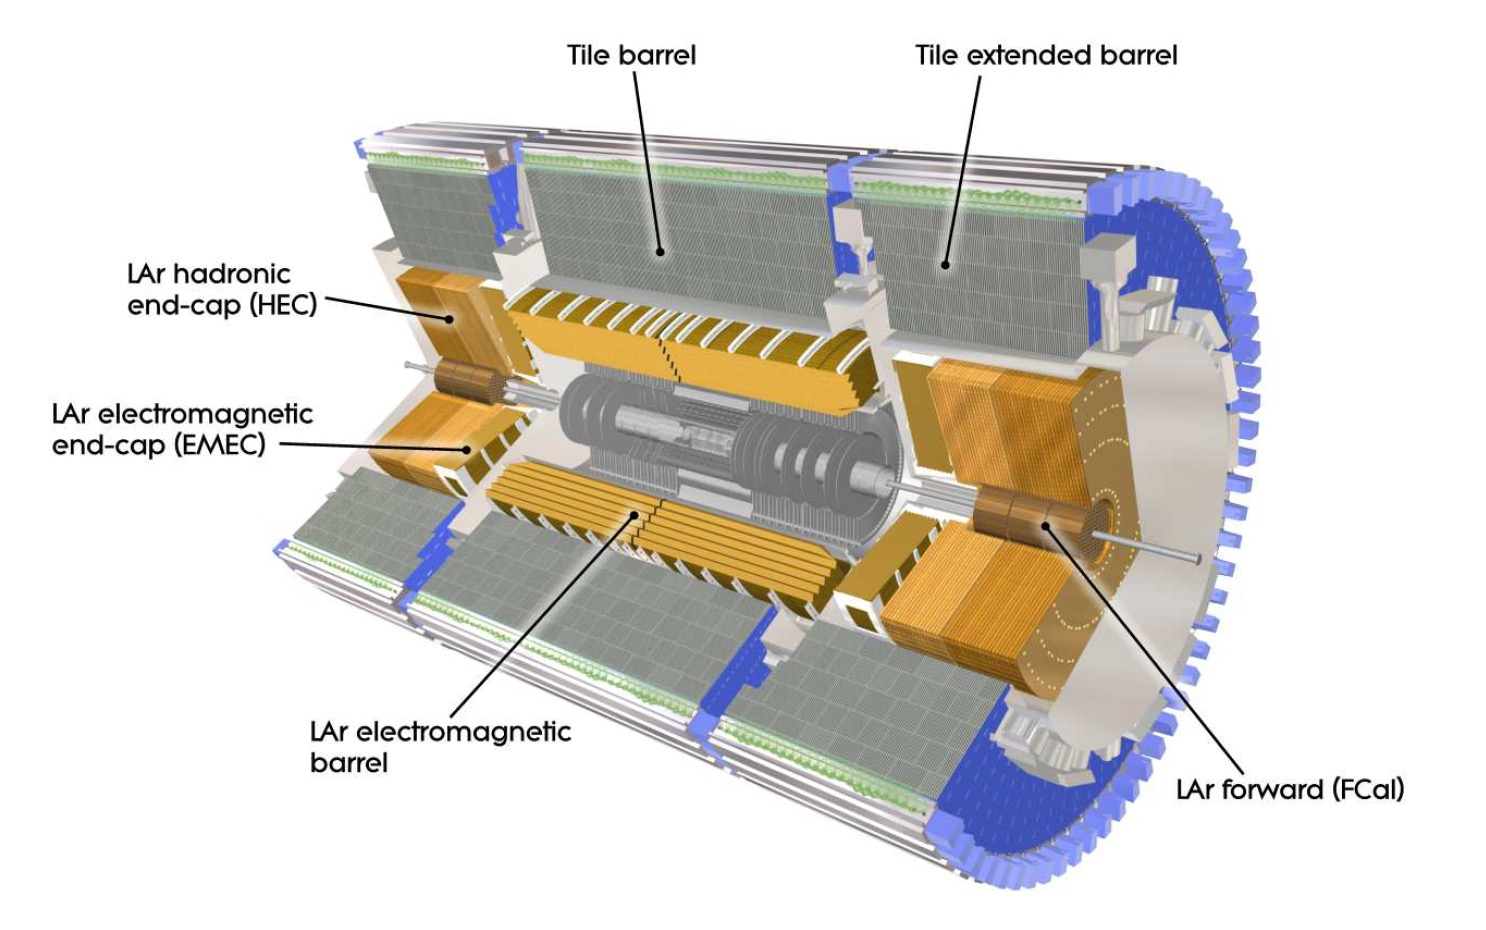
\includegraphics[width=0.75\textwidth]{figuresEXP/ATLASCA1.jpg}
  \end{center}
  \caption{
\textsc{ATLAS}探测器的量能器系统的截面图。
  }
    \label{fig:ATLASCA1}
\end{figure}

ATLAS的量能器系统使用的是采样式量能器,
如图~\ref{fig:ATLASCA2}所示,它们由吸收材料和活性材料交替组成。
其中吸收材料由铅、铜或者铁制成,用来降低入射粒子能量,
液氩或者乙烯闪烁体用作活性材料,通过电离或者闪烁收集可测量的信号,
利用测量的小部分能量可以推断出完整的簇射能量。

\begin{figure}
  \begin{center}
    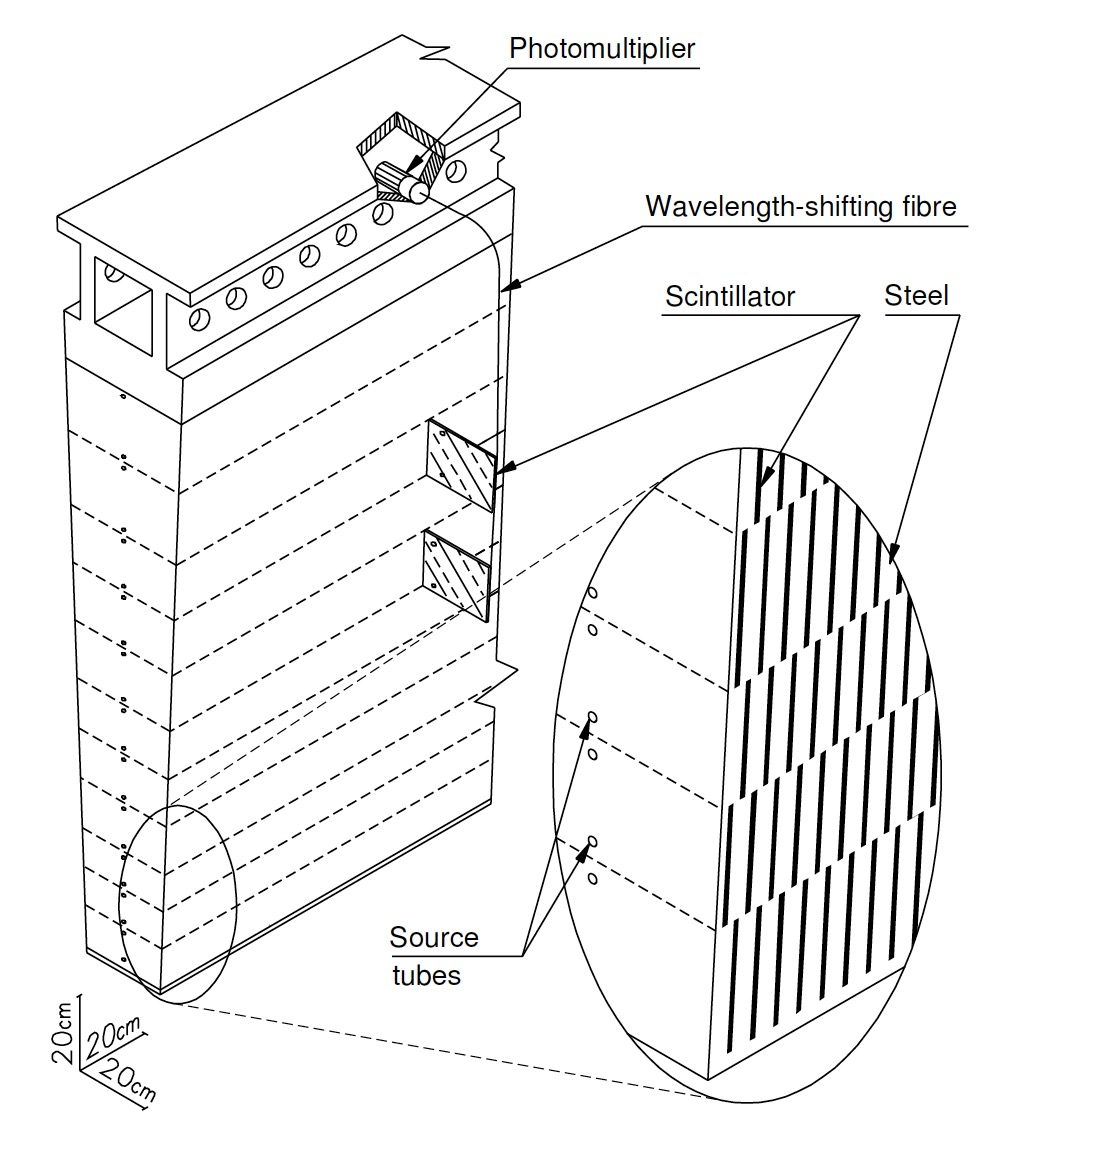
\includegraphics[width=0.75\textwidth]{figuresEXP/ATLASCA2.jpg}
  \end{center}
  \caption{
\textsc{ATLAS}的量能器的机械组件和读出系统的组装模式。
  }
    \label{fig:ATLASCA2}
\end{figure}

整个电磁量能器长6.65m,外径为2.25m,
分别由铅和液氩作为吸收材料和活性材料,并带有一个聚酰亚胺电极用于信号输出,
能量分辨率为:
\begin{equation} 
\label{eq:EMsigma1}
\frac{\sigma(E)}{E}=\frac{10\%}{\sqrt{E}}\oplus 0.7\%
\end{equation}
覆盖整个方位角$0\le\phi<2\pi$。
它可以分为桶部和左右端盖三个部分,分别覆盖了$|\eta|<1.475$和$1.375<|\eta|<3.2$的范围,
为了能够完整的包含入射电子和光子产生电磁簇射,
桶部和端盖的厚度分别大于22$X_0$和24$X_0$,
其中$X_0$为辐射长度,定义为粒子在其能量减小到初始能量的$1/e$之前所经过的平均距离,
可以用原子序数$Z$和原子质量数$A$近似的表示成~\cite{PDG}:
\begin{equation} 
\label{eq:X0def}
X_0=\frac{716.4A}{Z(Z+1)\ln(287/\sqrt{Z})}g cm^{-2}
\end{equation}
图~\ref{fig:ATLASCA3}是桶部电磁量能器的模块示意图,
第一层粒度较小,用于电子和光子的识别,
后面两层粒度较大,用以保证电子和光子产生的电磁簇射被完全吸收。

\begin{figure}
  \begin{center}
    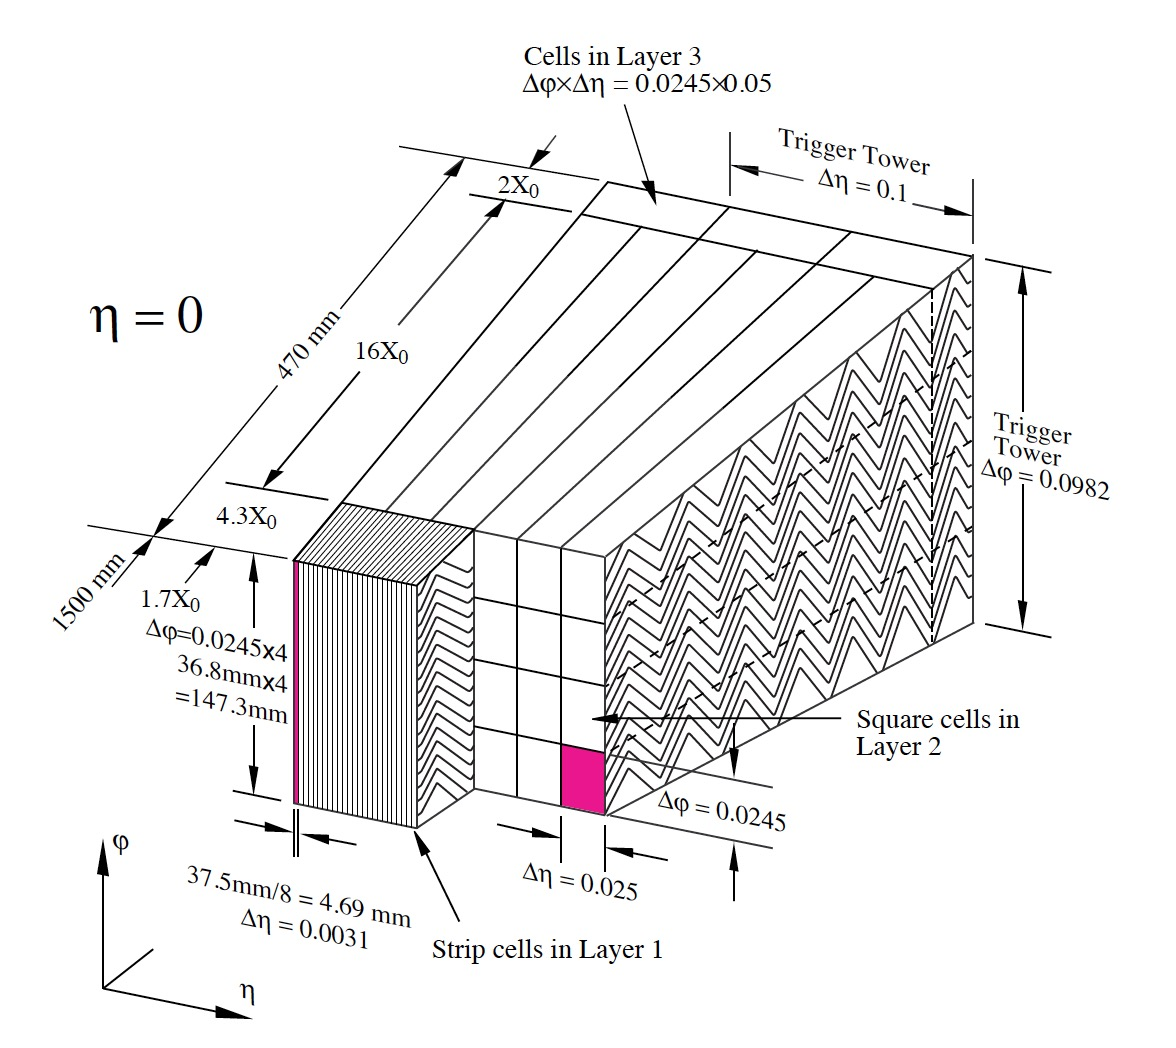
\includegraphics[width=0.75\textwidth]{figuresEXP/ATLASCA3.jpg}
  \end{center}
  \caption{
桶部电磁量能器的模块示意图。
  }
    \label{fig:ATLASCA3}
\end{figure}

强子量能器紧靠在电磁量能器外面,长6.10m,外径4.25m,
其能量分辨率为:
\begin{equation} 
\label{eq:EMsigma2}
\frac{\sigma(E)}{E}=\frac{50\%}{\sqrt{E}}\oplus 3\%
\end{equation}
同样由桶部和左右端盖三部分组成。
桶部强子量能器用铁和闪烁体分别作为吸收材料和活性材料,
粒度为$\Delta\eta\times\Delta\phi=0.1\times0.1$,
覆盖了$|\eta|<1.7$的部分。
而端盖强子量能器分别用铜和液氩作为吸收材料和活性材料,
粒度随着$\eta$变化,在$1.5<|\eta|<2.5$的范围为$\Delta\eta\times\Delta\phi=0.1\times0.1$
,在$2.5<|\eta|<3.2$的范围为$\Delta\eta\times\Delta\phi=0.2\times0.2$,
覆盖了$1.5<|\eta|<3.2$的部分。
图~\ref{fig:ATLASCA4}展示了端盖强子量能器在$R$-$\phi$平面和$R$-$z$平面的视图。

\begin{figure}
  \begin{center}
    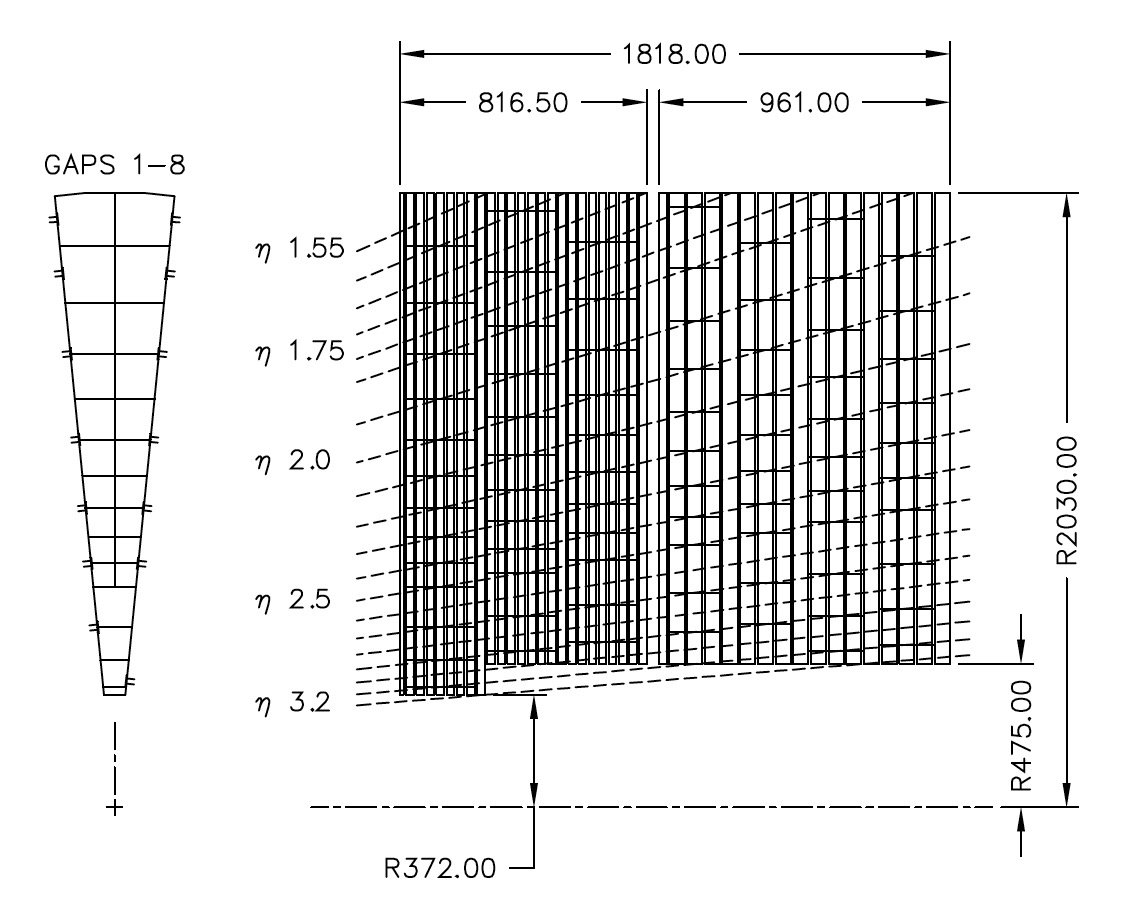
\includegraphics[width=0.75\textwidth]{figuresEXP/ATLASCA4.jpg}
  \end{center}
  \caption{
端盖强子量能器沿$R$-$\phi$平面和$R$-$z$平面的截面图,单位是mm。
  }
    \label{fig:ATLASCA4}
\end{figure}

前端量能器是一个组合型量能器,
能同时测量电磁簇射和强子簇射沉积的能量。
它距离对撞点仅4.7m,分为左右两个部分,覆盖了$3.1<|\eta|<4.9$,
能量分辨率为:
\begin{equation} 
\label{eq:EMsigma3}
\frac{\sigma(E)}{E}=\frac{100\%}{\sqrt{E}}\oplus 10\%
\end{equation}
由于所处位置的粒子通量较大,因此它采用了封闭式设计,
从而使粒子在各个量能器模块之间的隙缝中的能量损失降到最低,
还能限制簇射粒子到达$\mu$子谱仪。
如图~\ref{fig:ATLASCA5}所示,每个部分又可以分为三个紧密相连的模块:
依次是一个电磁量能模块(FCal1)和两个强子量能模块(FCal2, FCal3)。
三个模块都用液氩作为活性材料,
为了优化分辨率和能快速散热,电磁量能器用铜作为吸收材料。
强子量能模块用钨作为吸收材料,来防止来自强子簇射的粒子横向扩散出去并保证其封闭性。

\begin{figure}
  \begin{center}
    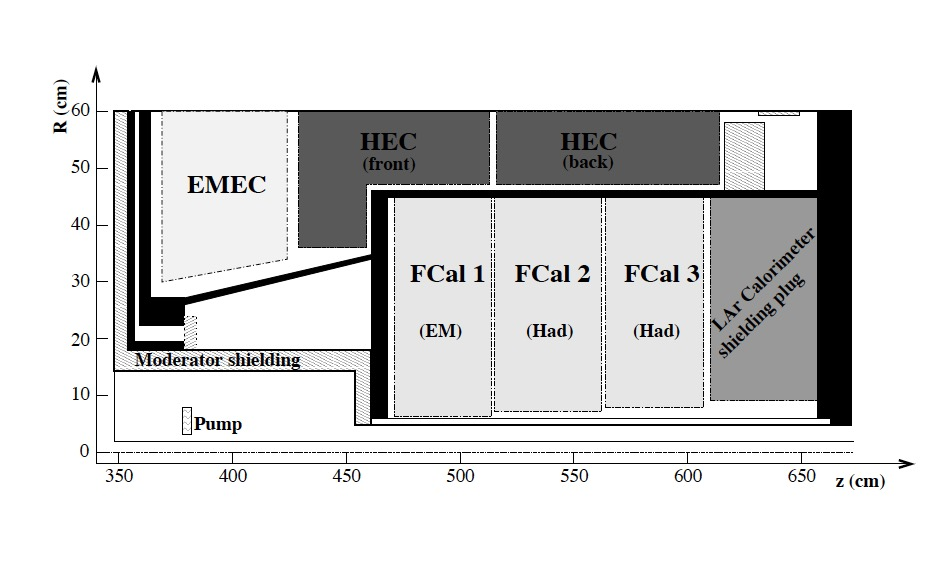
\includegraphics[width=0.75\textwidth]{figuresEXP/ATLASCA5.jpg}
  \end{center}
  \caption{
前端量能器的示意图。
  }
    \label{fig:ATLASCA5}
\end{figure}





\subsection{$\mu$子谱仪}
\label{sec:ATLASMS}

$\mu$子谱仪(the Muon Spectrometer, MS)~\cite{ATLASMUSPEC}位于ATLAS探测器的最外层,
由精密室(Precision Chambers)和触发室(Triggering Chambers)两大部分组成,从径向半径5m处延伸到接近10m的位置。
由于$\mu$子与量能器材料的相互作用截面极低,
它们在穿过量能器是仅丢失了很小一部分能量,能逃离量能器并被$\mu$子谱仪探测到。
精密室用于在$|\eta|<2.7$的范围内重建离开量能器的$\mu$子动量,
然后通过结合内部探测器中的信息,可以重建出来自对撞点的$\mu$子动量信息,
触发室能在$|\eta|<2.4$的范围快速触发$\mu$子的径迹。

精密室又由可监控漂移腔室(the Monitored Drift Tubes, MDT)~\cite{ATLASMDT}和阴极剥离腔室(the Cathode Strip Chambers, CSC)两部分组成。
可监控漂移腔室用于测量桶部覆盖的$z$坐标和端盖部分覆盖的$|\eta|<2.7$范围内的$\mu$子,
它的基本组件元是压力漂移管,直径为30mm,管内充满了处于3bar恒压的$Ar/CO_2$混合气体,
管壁作为阴极,管内中心有一根直径为50$\mu m$的钨铼合金丝作为阳极。
如图~\ref{fig:ATLASMS1}所示,$\mu$子穿过时使管内混合气体电离,产生的电子和正离子分别会向合金丝和阴极漂移,从而触发电信号。
整个精密室包含1150个可监控漂移腔室,可监控漂移腔室的平均分辨率为35$\mu m$($z$),且每个腔室由3到8层压力漂移管构成。
高横动量的$\mu$子动量测量精度取决于弧矢的分辨率,即$R$-$z$平面中$\mu$子圆弧径迹相对于弦的偏差,
对于横动量为1TeV的子,对应的弧矢大约为500$\mu m$。
而可监控漂移腔室对于横动量在10GeV和1TeV之间的$\mu$子的测量精度$\sigma_{p_{T}}/p_{T}$能达到$2\%$到$10\%$之间。

\begin{figure}
  \begin{center}
    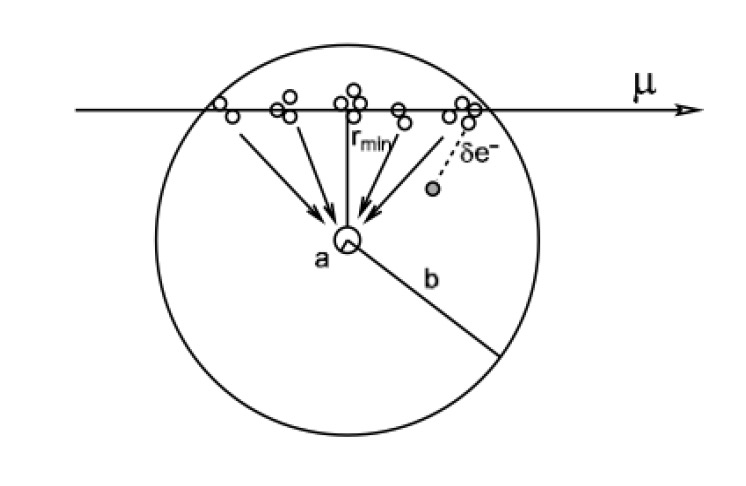
\includegraphics[width=0.5\textwidth]{figuresEXP/ATLASMS1.jpg}
  \end{center}
  \caption{
带电粒子穿过可监控漂移腔室中压力漂移管的截面图。漂移管中混合气体被带电粒子电离之后,产生的电子会向阳极漂移。
  }
    \label{fig:ATLASMS1}
\end{figure}

阴极剥离腔室是多线程腔室,如图~\ref{fig:ATLASMS2}所示,
它是由沿径向的带正电的阳极线阵和包围它们的带负电的铜质阴极组成,
其间充满了$Ar$、$CO_2$和$CF_4$混合气体,
用来测量前向区域$2<|\eta|<2.7$的范围内的$\mu$子动量。
整个精密室包含32个阴极剥离腔室,腔室的分辨率为$40\mu m\times5mm$($R\times\phi$)。

\begin{figure}
  \begin{center}
    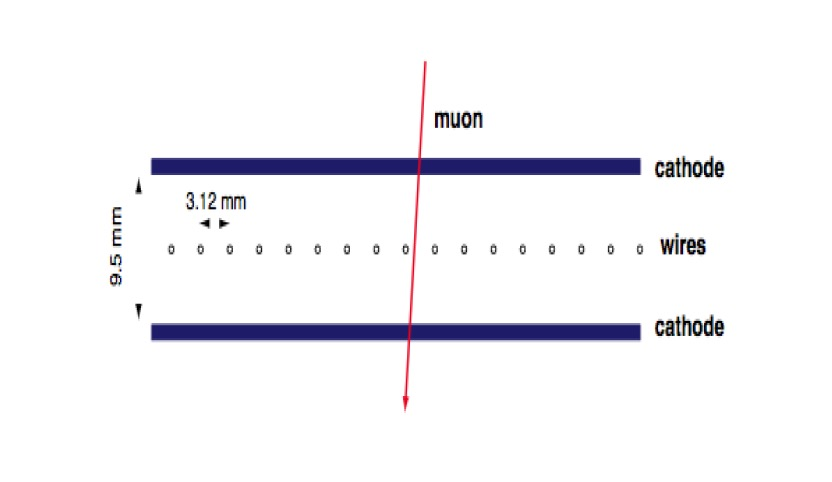
\includegraphics[width=0.6\textwidth]{figuresEXP/ATLASMS2.jpg}
  \end{center}
  \caption{
阴极剥离腔室的截面图。
  }
    \label{fig:ATLASMS2}
\end{figure}

$\mu$子谱仪非常重要的一个设计标准是其触发$\mu$子径迹的能力,
用以区分$\mu$子的多样性和近似的能量范围,
因此为了弥补精密室的功能,触发室用于$\mu$子触发,
它能在$\mu$子通过之后的几十纳秒内传递该$\mu$子的径迹信息。
触发室又分为电阻板腔室(the Resistive Plate Chambers, RPC)~\cite{ATLASRPC}和薄隙腔室(the Thin Gap Chambers, TGC)~\cite{ATLASTGC}。
其中电阻板腔室由两个高电阻率的平行塑料板组成,一个带正电的阳极和一个带负电的阴极,
两极板之间中间充满了$C_2H_2F_4$、$C_4H_{10}$和$SF_6$混合气体。
如图~\ref{fig:ATLASMS3}所示,每个极板有两个正交的读出信道:
$\eta$信道平行于可监控漂移腔室的阳极合金丝;
$\phi$信道垂直于可监控漂移腔室的阳极合金丝。
它覆盖了$|\eta|<1.05$的范围,其空间分辨率为$10mm\times10mm$($z\times\phi$),时间分辨率达到了1.5ns。

\begin{figure}
  \begin{center}
    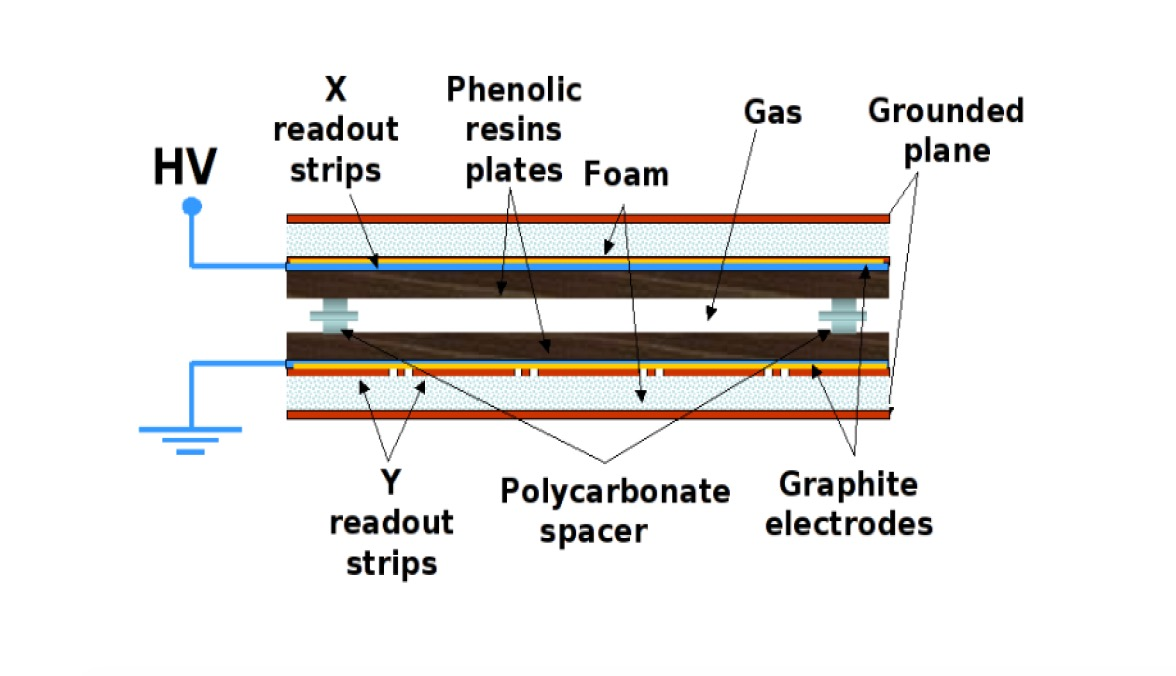
\includegraphics[width=0.6\textwidth]{figuresEXP/ATLASMS3.jpg}
  \end{center}
  \caption{
电阻板腔室结构简图。
  }
    \label{fig:ATLASMS3}
\end{figure}

薄隙腔室由两块作为阴极的接地电阻板和夹在其中的带有正高压的保持一定间隔的导线阵列组成,
如图~\ref{fig:ATLASMS4}所示,覆盖了$1.05<|\eta|<2.4$的范围。
阴极电阻板板之间是$CO_2$/n-$C_5H_{12}$混合气体。
阴极导线平行于可监控漂移腔室的阳极合金丝,并接有读出信道,能用于信号触发。
薄隙腔室同样具有非常好的时间和空间分辨率,其空间分辨率主要由阴极导线的数量决定。


\begin{figure}
  \begin{center}
    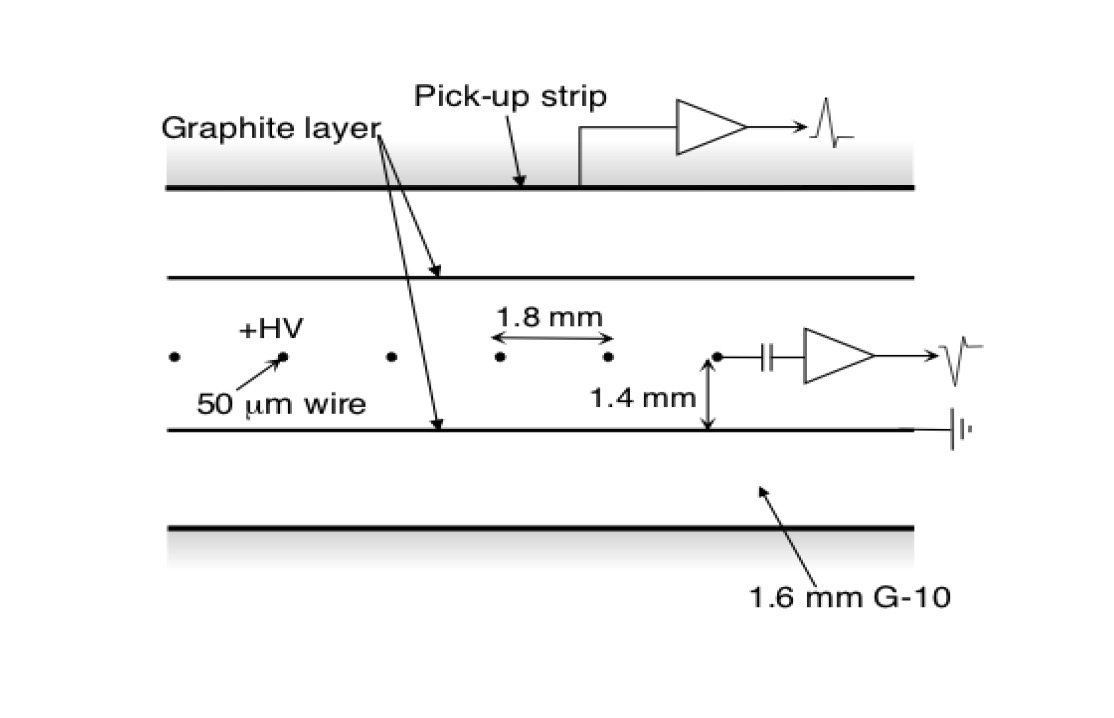
\includegraphics[width=0.6\textwidth]{figuresEXP/ATLASMS4.jpg}
  \end{center}
  \caption{
薄隙腔室的结构简图。
  }
    \label{fig:ATLASMS4}
\end{figure}

%图~\ref{fig:ATLASMS5}展示了$\mu$子谱仪在$x$-$y$平面和$z$-$y$平面的截面图,其内部结构和前述各个子探测器都有标注。
表~\ref{tab:ATLASTab2}总结了$\mu$子谱仪中各个子探测器的重要参数。

%\begin{figure}
  %\begin{center}
    %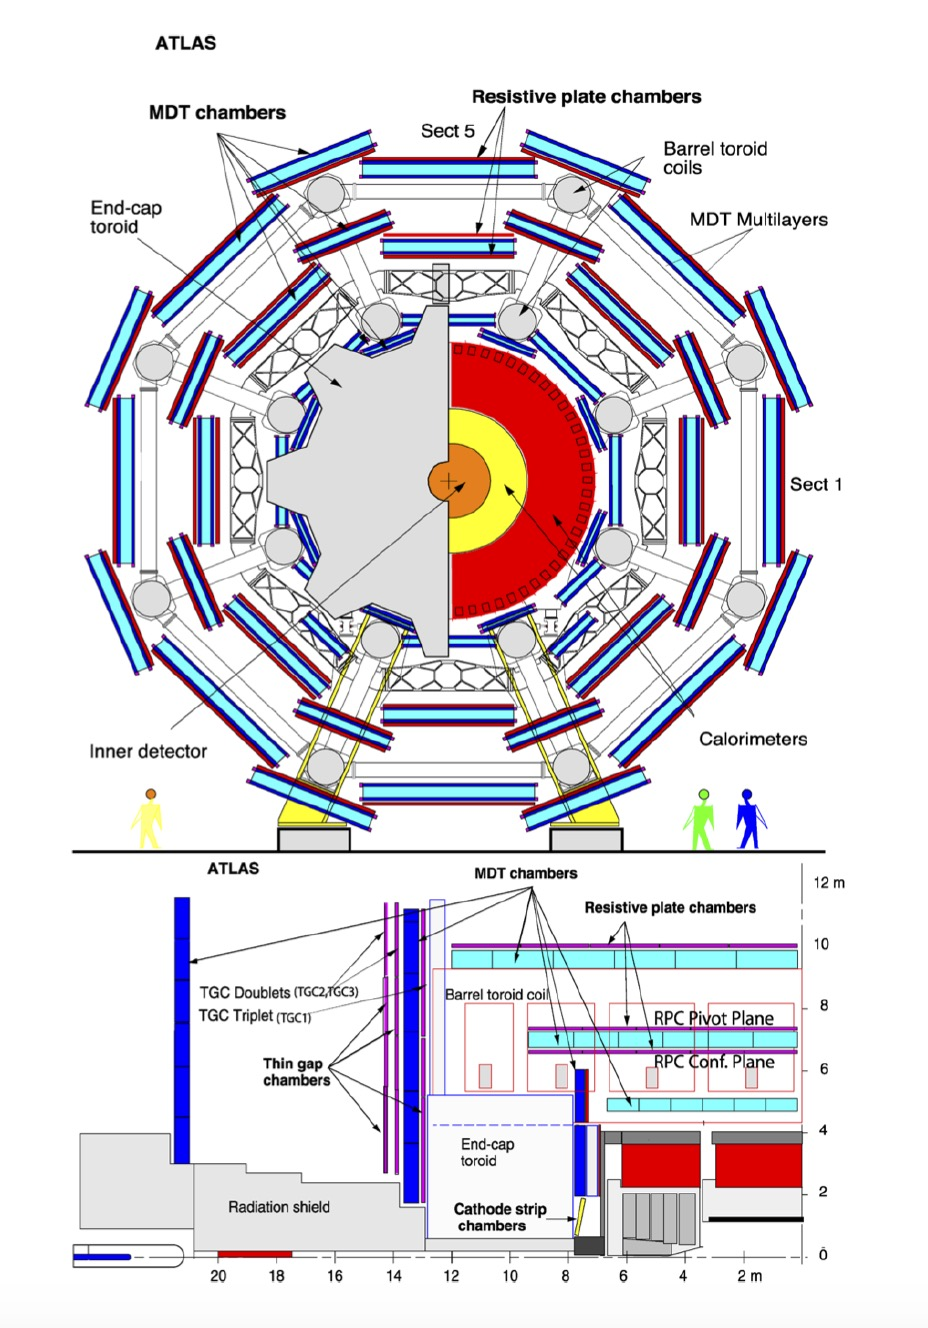
\includegraphics[width=0.75\textwidth]{figuresEXP/ATLASMS5.jpg}
  %\end{center}
  %\caption{
%$\mu$子谱仪在$x$-$y$平面(上)和$z$-$y$平面(下)的截面图。
 % }
   % \label{fig:ATLASMS5}
%\end{figure}

\begin{table}[htbp]
      \caption{
$\mu$子谱仪的四个子探测器的参数。      
      }
      \label{tab:ATLASTab2}
      \centering
      \begin{adjustbox}{width=\columnwidth,center}
      \begin{tabular}{|c|c|c|c|c|c|c|c|c|}
        \hline
         Type & Function  &   \multicolumn{3}{|c|}{Chamber resolution in}   &   \multicolumn{2}{|c|}{Measurements/track}   &   \multicolumn{2}{|c|}{Number of}  \\
         \hline
         &   &  $z/R$ & $\phi$  & time  & barrel  & end-cap  &  chambers &   channels \\
         \hline
         MDT& tracking  & 35$\mu m(z)$ & -  &  - & 20  &  20 & 1150  &  354k \\
         \hline
         CSC& tracking  & 40$\mu m(R)$  &  5mm &  7ns &  - &  4 & 32  & 30.7k  \\
         \hline
         RPC& trigger  &  10$mm(z)$ & 10mm  & 1.5ns  &  6 & -  & 606  &  373k \\
         \hline
         TGC& trigger  & 2-6$mm(R)$  & 3-7mm  & 4ns  &  - & 9  & 3588  &  318k \\
         \hline
      \end{tabular}
      \end{adjustbox}
\end{table}

\subsection{触发和数据采集系统}
\label{sec:ATLASTDAS}

触发和数据采集系统~\cite{ATLASTDAQ}是ATLAS探测器的重要组成部分,
它负责决定是否将庞大的数据中给定的碰撞事例保存下来作为一个值得研究的物理过程用于后续的离线分析。
$Run\_2$计划相对于$Run\_1$计划具有更高的亮度和对撞能量,
因此$Run\_2$计划之前,对ATLAS探测器的触发和数据采集系统进行了升级,
升级之后的系统能将质子束碰撞频率(the bunch crossing rate)高达40MHz的数据减小到1kHz并记录下来。

如图~\ref{fig:ATLASTS1}所示,
$Run\_2$计划整个触发系统~\cite{ATLASRTS}由基于硬件的一级触发器(First Level Trigger)和
基于软件的高级触发器(High Level Trigger)组成。
一级触发器有量能器一级触发和$\mu$子一级触发两种类型,
它可以访问粗粒度量能器和$\mu$子谱仪中的原始数据,
并基于粒子的多样性和$\mu$子横动量等信息作出决策,
进行事例的初始筛选。
一级触发器能将40MHz的质子束碰撞频率降低到100kHz,总延迟为2.5$\mu s$,
随后筛选出来的信息会被送到高级触发器,并将事例率降低到1kHz。
高级触发器用于进一步的离线筛选和对象重建,为后续的物理分析做准备。

\begin{figure}
  \begin{center}
    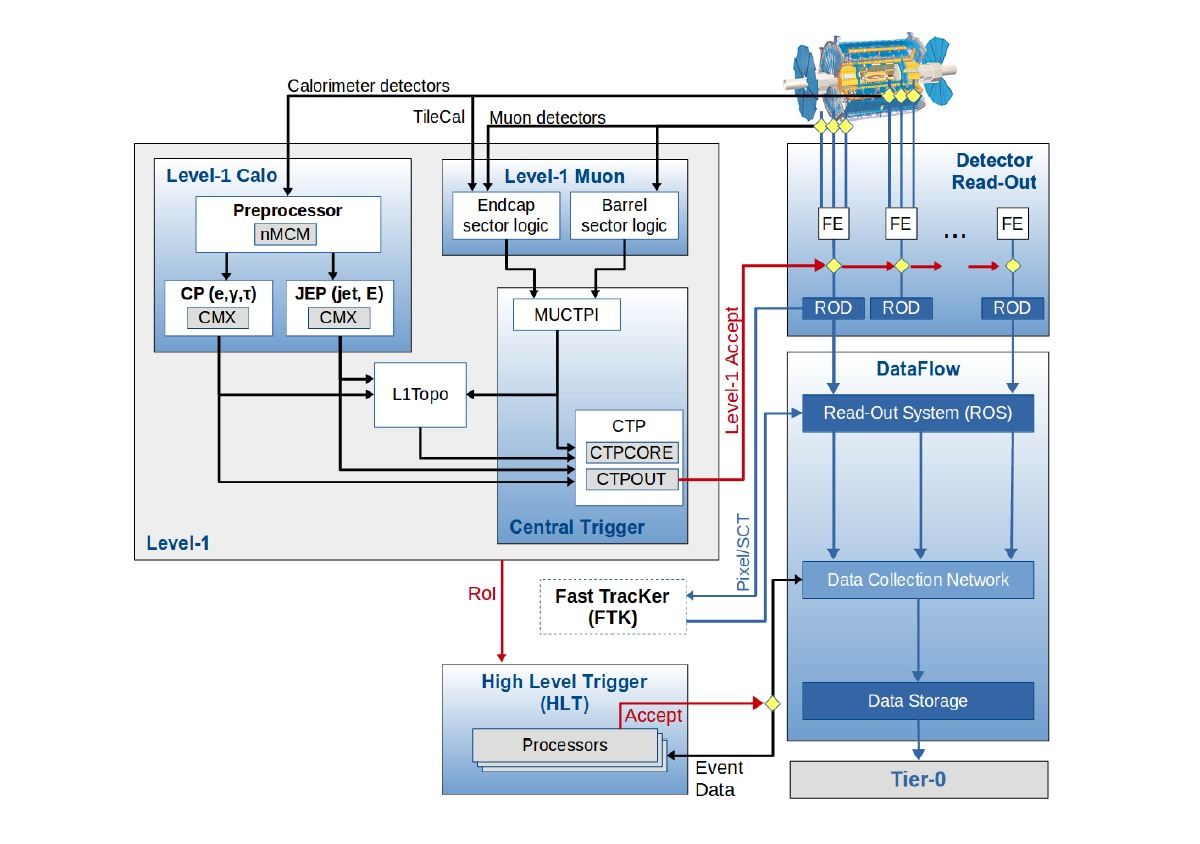
\includegraphics[width=0.75\textwidth]{figuresEXP/ATLASTS1.jpg}
  \end{center}
  \caption{
$Run\_2$计划的触发和数据采集系统的简图。
  }
    \label{fig:ATLASTS1}
\end{figure}

\subsection{亮度探测器系统}
\label{sec:ATLASLD}

ATLAS的亮度探测器系统~\cite{ATLASLUMID}用来测量亮度,并通过比较几个不同的亮度探测器的测量结果来确定亮度的误差。
如图~\ref{fig:ATLASLD1}所示~\cite{LDIm},整个系统位于ATLAS探测器前端,由切伦科夫亮度探测器(the Luminosity measurement using Cerenkov Integrating Detector, LUCID)、
零能探测器(the Zero-Degree Calorimeter, ZDC)和绝对亮度探测器(the Absolute Luminosity For ATLAS, ALFA)三个子探测器依次排列组成。
切伦科夫探测器离对撞点最近,仅$\pm 17m$,覆盖$5.6<\eta<6$的范围,
它可以通过在接收范围内计数每次对撞中产生的带电粒子数来计算非弹性质子-质子对撞的平均次数,从而监控前端的非弹性质子-质子散射率,它既可以测量积分亮度,也可以在线监控瞬时亮度。
零能探测器位于离对撞点$\pm 140m$、$8.3<\eta$的位置,
它主要通过探测对撞过程中产生的正向中子来测量相对亮度,
它可以测量质子-质子对撞的亮度,也可以测量重离子对撞的亮度,
绝对亮度探测器距离对撞点$\pm 240m$,覆盖的范围是$10.6<\eta<13.5$,
它是由闪烁体纤维构成,通过在小角度上探测质子-质子散射来确定绝对亮度和总的质子-质子散射截面。

\begin{figure}
  \begin{center}
    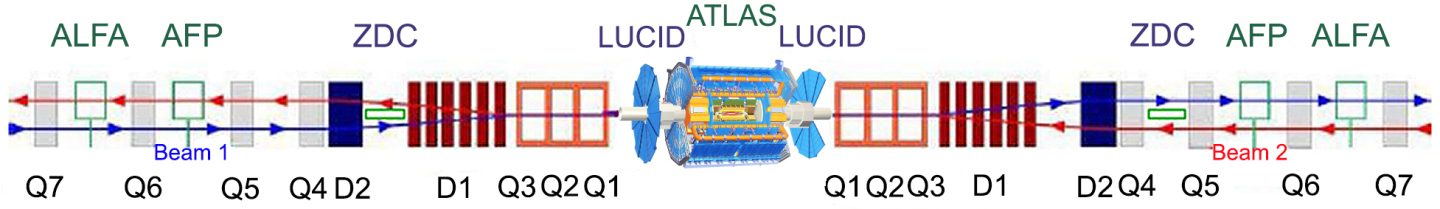
\includegraphics[width=0.98\textwidth]{figuresEXP/ATLASLD1.jpg}
  \end{center}
  \caption{
ATLAS的亮度探测器系统。
  }
    \label{fig:ATLASLD1}
\end{figure}


\section{MC模拟}
\label{sec:Simulation}

为了使用理论模型对实验结果作出准确的预测,
对碰撞事例的产生及粒子与探测器的相互作用过程进行精确的Monte Carlo模拟简称MC模拟是高能物理领域非常关键的一步。
ATLAS合作组有一套模拟系统~\cite{ATLASMC},
可以用于实验分析的许多方面,包括对标准模型的预测、校准、分析优化和系统误差的确定等,
本章将做简要介绍。

\subsection{硬散射和部分子簇射}
\label{sec:MCHS}

MC模拟中关键的一环是对被模拟的硬散射过程的截面的计算。
截面的计算依赖于QCD因式分解定理~\cite{MC1},
利用部分子分布函数(Parton Distribution Functions, PDFs)~\cite{MC2},
该定理可以将低动量部分子相互作用与部分子硬散射过程分离。
其中不参与硬散射过程的低动量部分子相互作用产生的事例被称为潜在事例(the underlying event)~\cite{MC3},
而部分子硬散射过程的截面与矩阵元的平方成正比,
对于这部分,可以使用微扰论对相互作用的耦合常数进行展开,
从而展开后的有限项用于近似部分子硬散射的截面,
并且展开后的每一项都可以用费曼规则~\cite{FEYNR}进行计算。

%\subsection{部分子分布函数和部分子簇射}
%\label{sec:MCPDF}
其中部分子分布函数是一个经验式的函数,
从不同的实验合作组可以得到不同的形式。
它给出了部分子占入射质子纵向动量比例的概率,
并且依赖于硬散射过程中的动量传递,
通过它可以实现质子的动量和参与硬散射过程的部分子动量之间的转换。
部分子发生硬散射前后,都可以辐射其他部分子,这个过程称为部分子簇射,
它和硬散射过程一起可以由部分子簇射模拟器来模拟~\cite{MC6}。


\subsection{强子化}
\label{sec:MCHARD}
如第~\ref{cha:Theory}~章所述,由于色禁闭的影响,
夸克或胶子在产生之后会通过强子化形成不带色荷的强子束缚态,
并且QCD中渐近自由的性质使得强子化过程不能用微扰近似来计算,
即无法从第一性原理来解释这个过程,从而需要建模来描述强子化。
现在,强子化建模的主流模型有两个:Lund弦模型(the Lund string model)~\cite{Hadonization}和簇模型(the cluster model)~\cite{MC4}。
其中在Lund弦模型中,如图~\ref{fig:MC1}所示,夸克通过随着夸克分离而拉伸的弦连接在一起,
这些弦可以被拉断,同时能在新弦的末端产生一个夸克-反夸克对,
这个过程一直持续到能量不足以拉断弦并且所有弦都通过断裂形成了强子为止。

这种模型的强子化过程可以由部分子簇射模拟器\textsc{Pythia}~\cite{MC5}来模拟完成,
它可以同时用于事例产生和矩阵元产生。
接下来便是矩阵元的计算和模拟不稳定强子的衰变过程,
它们分别可以由\textsc{MadGraph5}~\cite{Alwall:2014hca}和\textsc{Evtgen}~\cite{Lange:2001uf}来模拟实现。
%其他不稳定粒子的衰变可以在\textsc{Pythia}内完成。

\begin{figure}
  \begin{center}
    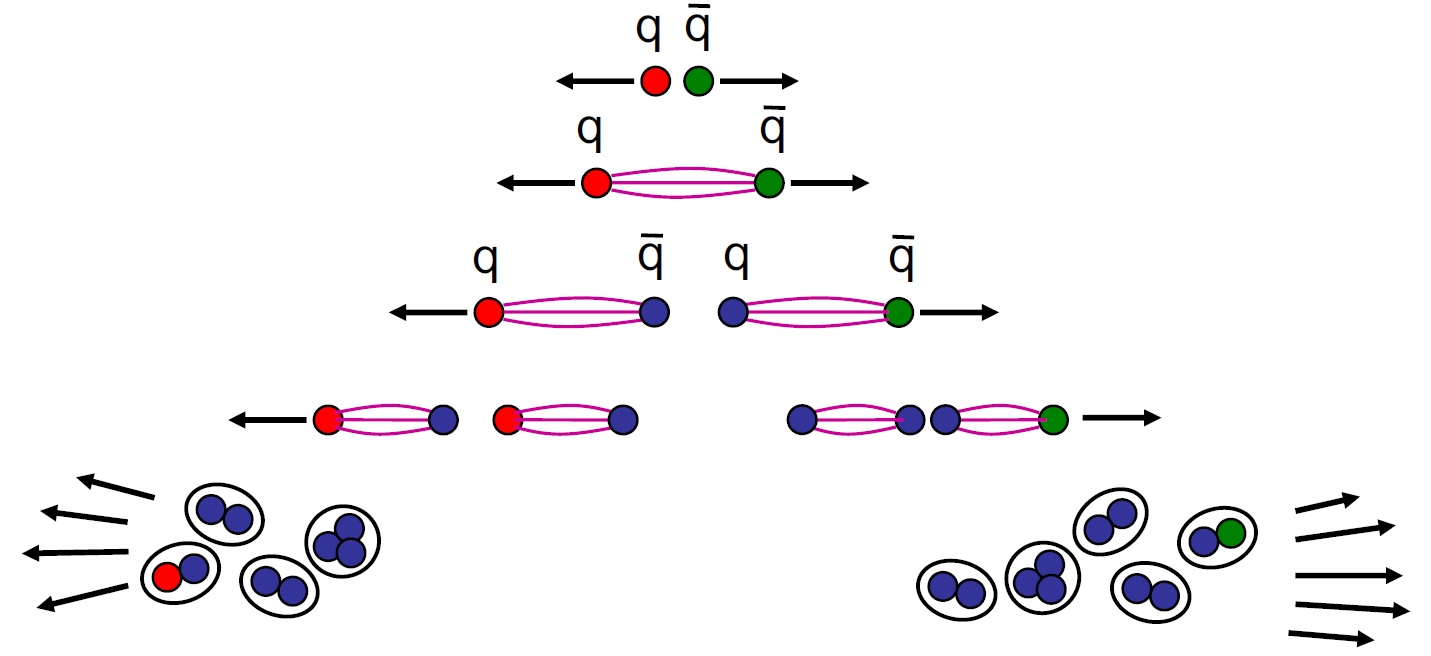
\includegraphics[width=0.9\textwidth]{figuresEXP/MC1.jpg}
  \end{center}
  \caption{
Lund弦模型的强子化过程。
  }
    \label{fig:MC1}
\end{figure}


\subsection{探测器模拟}
\label{sec:MCDET}

所模拟的质子-质子对撞产生的粒子与探测器的相互作用和最终的电子学输出是通过\textsc{Geant4}~\cite{MC7}模拟的,
它能准确模拟ATLAS探测器中的各种探测器材料与其几何形状,并精确的重现粒子与探测器材料的相互作用行为。
传统的模拟过程以非常精确的方式模拟探测器的响应,对可能影响粒子的任何微小结构都会进行建模,称为全模拟(Full simulation),
这种方法非常耗时,也耗费资源。
因此,为了节省时间和资源,同时满足不同粒子在不同研究中的重要程度和对不同子探测器的精度要求,
构建了一种称为快模拟~\cite{MC8}的方法,
它能通过参数化对探测器材料和有源探测器元件的响应进行建模,
这种方法的明显缺点是精读降低了,但对于某些研究过程的粒子响应是可以接受的。


\section{物理对象的重建}
\label{sec:Reconstruction}

数据采集完成之后,便是重建用于实际物理分析的基本物理对象。
硬散射(hard-scattering)事例产生的粒子中仅有一小部分寿命足够长到能被ATLAS探测器探测到,
大部分粒子产生之后都会通过衰变或级联衰变成更轻、更稳定的粒子,进而被探测器探测到。
在已知的所有基本粒子和复合粒子中,只有十四种粒子的平均自由程大于500$\mu m$,
从而能与探测器材料相互作用并被探测到,它们是$\mu$子($\mu^+$, $\mu^-$)、电子($e^+$, $e^-$)、光子($\gamma$)、
$\pi$介子($\pi^+$, $\pi^-$)、K介子($K^+$, $K^-$, $K_L^0$)、质子($p^+$, $p^-$)和中子($n^+$, $n^-$)。
由于强相互作用具有色禁闭的性质,夸克或胶子产生之后会经过强子化过程~\cite{Hadonization}形成色中性的强子束缚态,
并在探测器中产生高度准直的强子簇射,被称为喷注或jet~\cite{JETS},其中包含有b强子的jet具有独特的性质,记为b-jet,
上述九种强子便是夸克或胶子在强子化过程中产生的。
由于中微子仅参与弱相互作用,而且作用截面极小,因此不能被ATLAS探测到,
它的存在是通过事例整体的横动量平衡来推断的,即丢失横动量的重建。
$\tau$子的寿命为$2.9×10^{−13}s$,在进入内部探测器之前会衰变,可以通过它的衰变产物来重建。
接下来会简要介绍一下这些物理对象的重建过程。


\subsection{径迹和顶点的重建}
\label{sec:TRACKS}

径迹可以用来识别碰撞产生的粒子和碰撞顶点,
它是通过使用一系列算法从粒子在内部探测器中留下的信息中重建的~\cite{TRACK1}。
首先,将带电粒子在PD和SCT探测器部分结构中留下的电信号转化成三维的空间位置信息。
如图~\ref{fig:ATLASORT1}所示,由单个带电粒子形成的点簇称为单粒子点簇,
由多个带电粒子形成的点簇称为合并点簇,合并点簇的识别和分离是通过一个基于机器学习的集群算法实现的~\cite{NNCLUSTER}。
然后通过三维空间位置信息中的每三个点构建径迹种子池,
其中它们的动量和碰撞参数必须满足一定的筛选条件,
而且种子池中每条径迹必须要有与之兼容的第四个点。
随后通过结合与种子池中径迹兼容的来自PD和SCT探测器其他结构中的空间位置信息,
利用\textsc{KalmanFilter}~\cite{KALMAN}从径迹种子池中构建候选径迹。
候选径迹构建完成之后,会引入一个解决歧义的算法来修正部分径迹的所属点有重叠或者分配错误的问题。
最后,便是对候选径迹中的点进行高分辨率的拟合。

\begin{figure}
  \begin{center}
    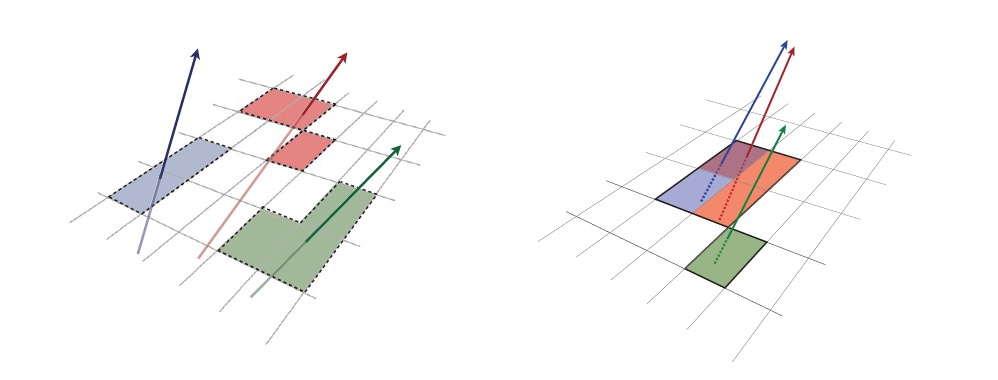
\includegraphics[width=0.9\textwidth]{figuresEXP/ATLASORT1.jpg}
  \end{center}
  \caption{
像素传感器上单粒子点簇(左)和合并点簇(右)示意图。
  }
    \label{fig:ATLASORT1}
\end{figure}


质子-质子硬散射的起点也就是主顶点的重建~\cite{VERTEX1,VERTEX2}对于实际的物理分析来说至关重要,
它不仅有助于后续物理对象的重建,还能有效的压低堆积事例~\cite{PileUp}。
主顶点是利用在内部探测器中重建出来的径迹重建出来的。
首先按一定条件从候选径迹中筛选出来一部分用于顶点重建,
并为这些满足条件的径迹分配一个候选顶点,
然后通过对候选顶点和径迹进行一个迭代拟合过程来寻找最优的顶点位置,
随后与这个最优顶点不相关联的径迹会被挑出来用于确定下一个顶点,
重复之前的操作,直到所有径迹都有与之关联的顶点或者在剩下的径迹中不能找到更多的顶点。

\subsection{量能器中拓扑集群的重建}
\label{sec:TOPTCLUS}


拓扑集群~\cite{TOPOCLUSTER}用于寻找量能器中来自硬散射过程的高能粒子的能量沉积,
同时抑制来自于电子元件和堆积事例的噪声。
这里引入量能器单元的能量沉积信噪比$\varsigma_{cell}$用于后续拓扑集群的重建,
它被定义为:
\begin{equation} 
\label{eq:TOPOSN}
\varsigma_{cell}=\frac{E_{cell}}{\sigma_{noise,cell}}
\end{equation}
其中$E_{cell}$是量能器单元中沉积的能量,$\sigma_{noise,cell}$是量能器单元中噪声的期望值。
首先选取满足$|\varsigma_{cell}|>4$的量能器单元作为种子集群,
然后与种子集群相邻的满足$|\varsigma_{cell}|>2$的量能器单元会被添加到临近的种子集群当中,构成新的种子集群,
这个过程会被重复,直到没有这样的临近量能器单元。
这样的重建过程是在三维尺度上完成的,
因此单个集群中的单元可能位于同一个量能器的同一模块,
也可能位于同一个量能器的不同模块或者不同的量能器。
最后所有与种子集群相邻的满足$|\varsigma_{cell}|>0$的量能器单元都会被合并到相对应的种子集群当中,
到此,拓扑集群的重建便完成了。
最后一个过程可能导致集群合并,
如果一个集群内存在着明显的局部能量最大,
那么将会有另一种算法对其进行拆分~\cite{TOPOCLUSTER}。
如图~\ref{fig:ATLASORT2}所示,在$Run\_1$计划中用MC模拟的事例在前端量能器第一个模块中重建出来的拓扑集群示例图。

\begin{figure}
  \begin{center}
    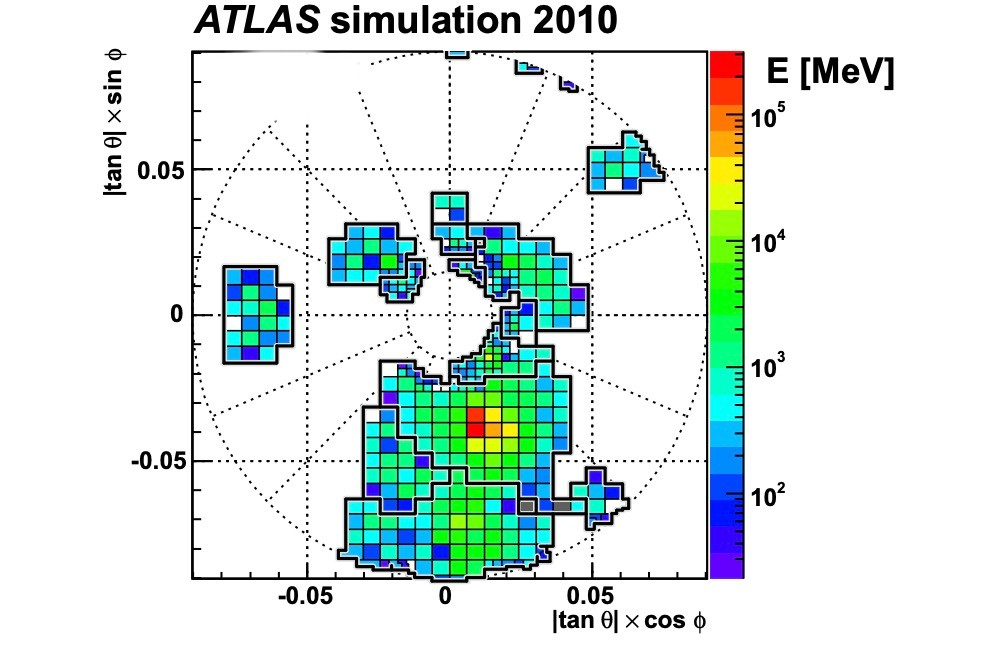
\includegraphics[width=0.75\textwidth]{figuresEXP/ATLASORT2.jpg}
  \end{center}
  \caption{
用MC模拟的事例在前端量能器第一个模块中重建出来的拓扑集群示例图。
  }
    \label{fig:ATLASORT2}
\end{figure}




\subsection{Jet的重建}
\label{sec:JET}

夸克或胶子强子化之后以圆锥形粒子簇射的形式被探测器探测到,即jet。
jet中带电粒子可以在内部探测器中留下径迹信息,
随后连同jet中其他粒子一起沉积在电磁量能器和强子量能器中,
因此,jet一般是从量能器的拓扑集群中重建出来的。
如图~\ref{fig:ATLASJET1}所示,首先,是在量能器系统中重建拓扑集群,这个过程在上一小节已有讨论。
随后通过应用$anti$-$k_t$~\cite{ANTIKT}算法进行jet重建,
该算法定义了一个拓扑集群之间的距离度量$d_{ij}$和一个拓扑集群与束流之间的距离度量$d_{iB}$:
\begin{equation} 
\label{eq:TOPOSN}
\begin{aligned}
d_{ij}=min\left( p_T^{2a}(i),p_T^{2a}(j) \right)\frac{\Delta R_{ij}^2}{R^2}
\\
d_{iB}=p_T^{2a}(i)
 \end{aligned}
\end{equation}
其中$p_{T}(i)$和$p_{T}(j)$分别是集群i和集群j的横动量,如式~\ref{eq:DRdef}中的定义,$\Delta R_{ij}$是集群i和集群j在$\eta$-$\phi$平面的距离,$a=-1$,$R$为距离参数。
对于每个集群i,比较两种度量$d_{ij}$和$d_{iB}$的大小,如果$d_{ij}$较小,则将集群i和集群j合并到单个中间集群中,
如果$d_{iB}$较小,那么集群i被确定为一个jet并从集群集合中移除,重复之前的操作直到这个集合中没有集群为止。
利用量能器拓扑集群将jet重建完之后,
通过一个称为“幻影”关联的算法~\cite{Cacciari:2008gn}将内部探测器中带电粒子的径迹与jet匹配起来,
其中“幻影”是指径迹的横动量被设置成无穷小之后的四矢量,
基本只保留了径迹的方向信息,
然后重新用anti-$k_t$算法将这个“幻影”和构成jet的量能器拓扑集群重新会聚到这个jet中,
这样保证了重建出来的jet仍然是之前的jet,
如果此时“幻影”也是jet的组成部分,那么相应的径迹就和jet匹配上了。


\begin{figure}
 \begin{center}
    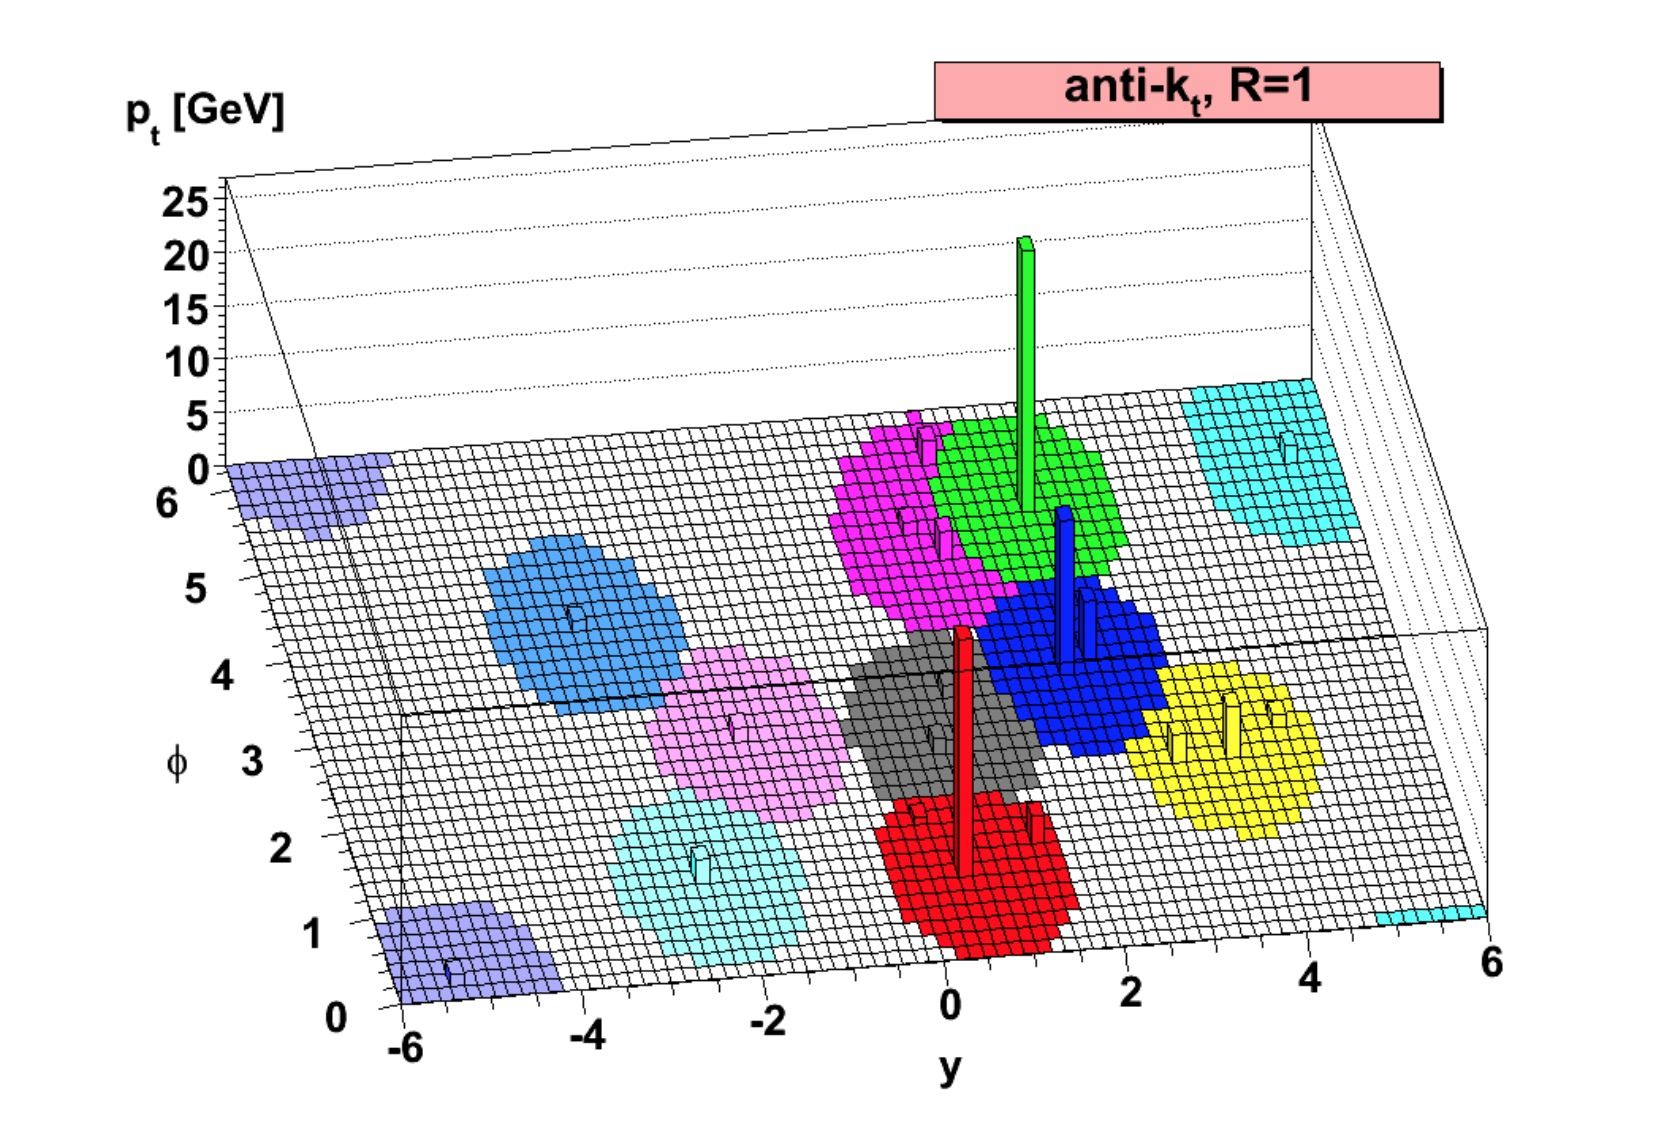
\includegraphics[width=0.75\textwidth]{figuresEXP/ATLASJET1.jpg}
  \end{center}
  \caption{
使用$anti$-$k_t$算法进行jet重建的示例图。彩色区域表示该算法重建出来的jet。
  }
    \label{fig:ATLASJET1}
\end{figure}


常用的固定的距离参数R有两个:使用R=0.4进行重建的jet代表夸克或胶子强子化在探测器中形成的jet,
记为SR-jet,章节~\ref{cha:Dijet}~中物理分析所使用的jet便是SR-jet;
而使用$R=1$进行重建的jet代表强子型衰变的高横动量且大质量粒子比如说希格斯玻色子在探测器中所形成的jet,
记为LR-jet,这是章节~\ref{cha:Xbb}~中新标定算法开发使用的一种jet;
%用$R=0.2$进行重建的jet代表包含在LR-jet中的小半径jet,记为FR-jet,章节~\ref{cha:Xbb}~中算法对比有用到这类jet。
%另外,合作组还引入了一种距离参数R可变的jet重建算法~\cite{VRJET1,VRJET2},记为VR-jet,
%在这个算法中,距离参数R是jet横动量$p_T$的函数:
%\begin{equation} 
%\label{eq:VR}
%R_{eff}(p_{T})=\frac{\rho}{p_T}
%\end{equation}
%其中新参数决定了有效的jet尺寸大小随着这个jet横动量动量减小的速度,
%除了之外,该算法还有两个附加的参数和分别对jet大小的上限和下限进行限制,
%这个限制可以防止jet在低横动量时变得太大或者在高横动量时收缩到探测器分辨率以下。
%这也是章节~\ref{cha:Xbb}~中新标定算法开发所使用的一种jet。
%FR-jet和VR-jet通常用于包含在LR-jet中的小半径jet,记为subjet的重建,
%如图~\ref{fig:ATLASJET2}~展示了利用FR-jet和VR-jet算法重建LR-jet中的subjet的简要示意图。


%\begin{figure}
  %\begin{center}
    %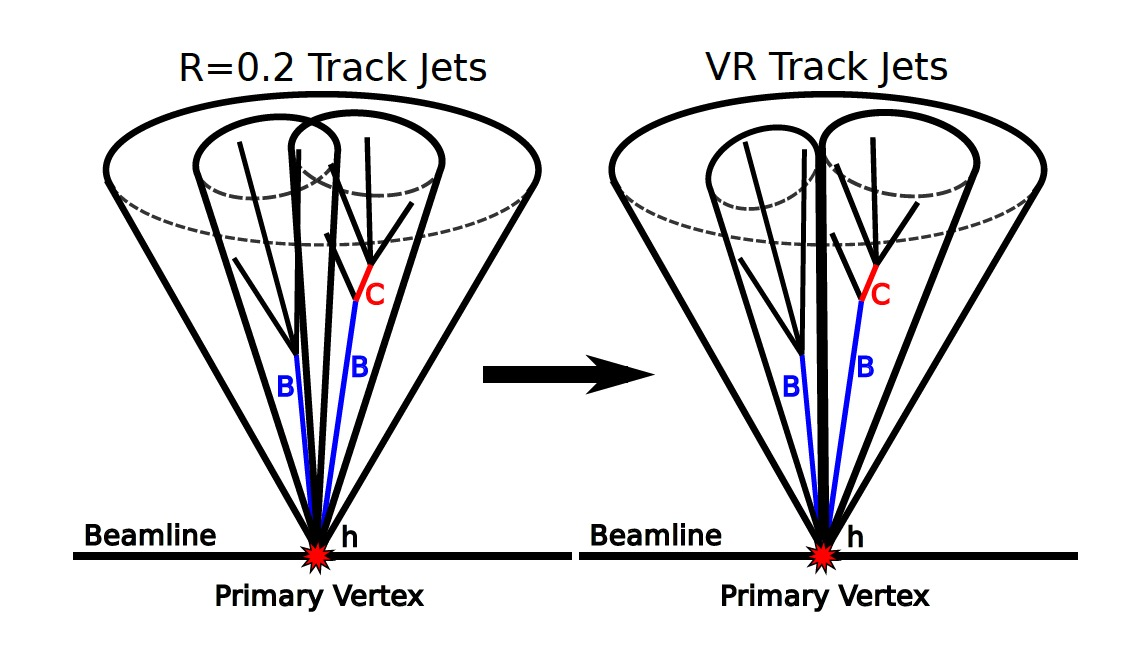
\includegraphics[width=0.9\textwidth]{figuresEXP/ATLASJET2.jpg}
  %\end{center}
  %\caption{
%使用固定半径$R=0.2$和可变半径重建LR-jet中的小半径jet的示意图。
  %}
    %\label{fig:ATLASJET2}
%\end{figure}


由于jet是一个由多粒子簇射重建出来的非常复杂的对象,
因此需要通过参考其他对象和模拟探测器响应来校准它的能量。
如图~\ref{fig:ATLASJET3}所示,jet能量的校准主要分为以下几步~\cite{JES1}:
首先将jet的方向校准到指向事例的主顶点,而不是探测器的中心,这样能显著提高$\eta$的分辨率~\cite{JES2};
然后基于jet在$\eta$-$\phi$平面的覆盖的区域和该区域中jet的横动量密度,
从jet能量中移除来自相同和相邻质子束中堆积事例的贡献~\cite{JES3}。
接着基于MC模拟的真实信息中主顶点的径迹数量和堆积事例率,修正jet能量~\cite{JES4};
接着在包含在jet中粒子的层面上校准jet的绝对能量~\cite{JES2};
随后结合量能器和内部探测器中的观测量进一步校准jet能量,
称为全局顺序校准~\cite{JES5},这一步消除了jet能量对味道信息和jet内部能量分布的依赖性;
最后是原位校准,用来解决数据和MC模拟中jet能量不匹配的问题~\cite{JES1}。

\begin{figure}
  \begin{center}
    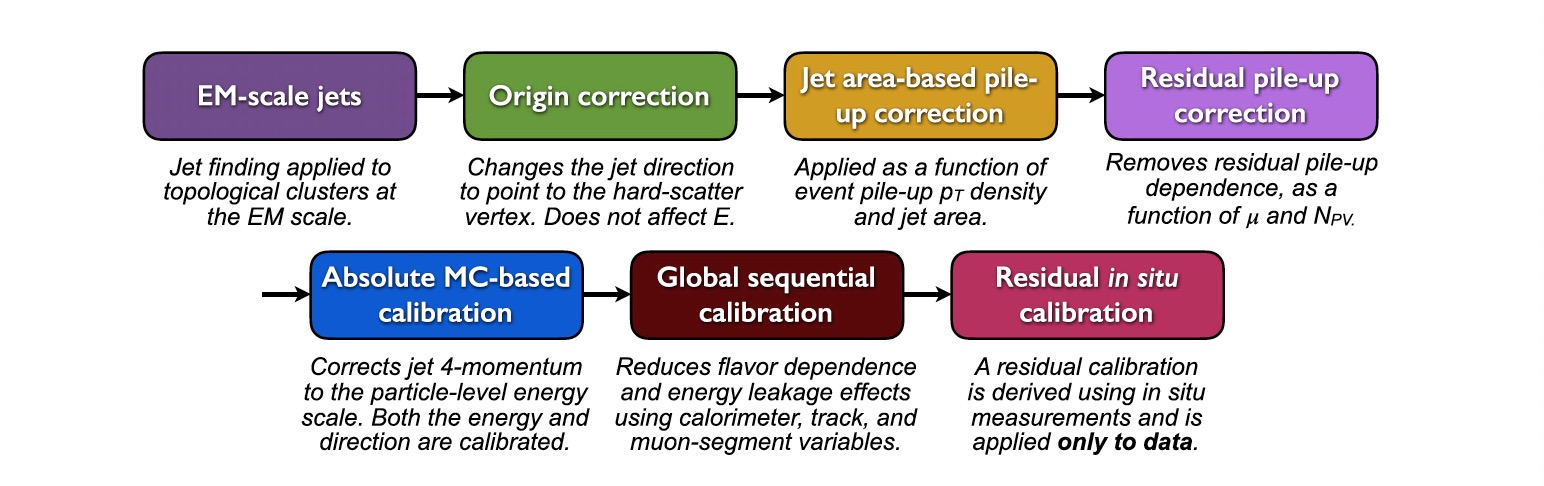
\includegraphics[width=0.9\textwidth]{figuresEXP/ATLASJET3.jpg}
  \end{center}
  \caption{jet能量校准流程图。 }
    \label{fig:ATLASJET3}
\end{figure}



\subsubsection{b-jet}
\label{sec:BJET}

相对于源于其他夸克的jet来说,来自b夸克的jet具有独特的性质,记为b-jet。
如图~\ref{fig:ATLASBJET1}所示,b夸克强子化之后,产生的b强子寿命比较长,约为$1.5\times10^{-12}s$,在ATLAS内部探测器中有明显的飞行距离,
使得可以通过离硬散射主顶点有一小段位移的第二顶点来识别b-jet。
ATLAS合作组中的b-jet鉴定过程~\cite{BTAGGING}分为两步,
第一步是重建b-jet中b强子的衰变特征,这个过程包含三个低级算法:
\begin{itemize}
	\item 利用b强子衰变径迹的碰撞参数构建\textsc{IP2D}和\textsc{IP3D}算法~\cite{IPTD};
	\item 用\textsc{SV1}算法~\cite{SVN}重建来自b强子衰变的第二顶点信息;
	\item 算法\textsc{JetFitter}~\cite{JETFT}可以完整的重建jet中b强子或c强子衰变链,因此可以用于b-jet中b强子衰变链的重建。
	%\item 利用递归神经网络发掘b强子衰变径迹之间的空间和运动学关联性的\textsc{RNNIP}算法~\cite{IPTD};
\end{itemize}
第二步是将这些互补算法的输入合并到一个机器学习算法中去,可以得到功能更强大的b-jet标定高级算法,


\begin{figure}
  \begin{center}
    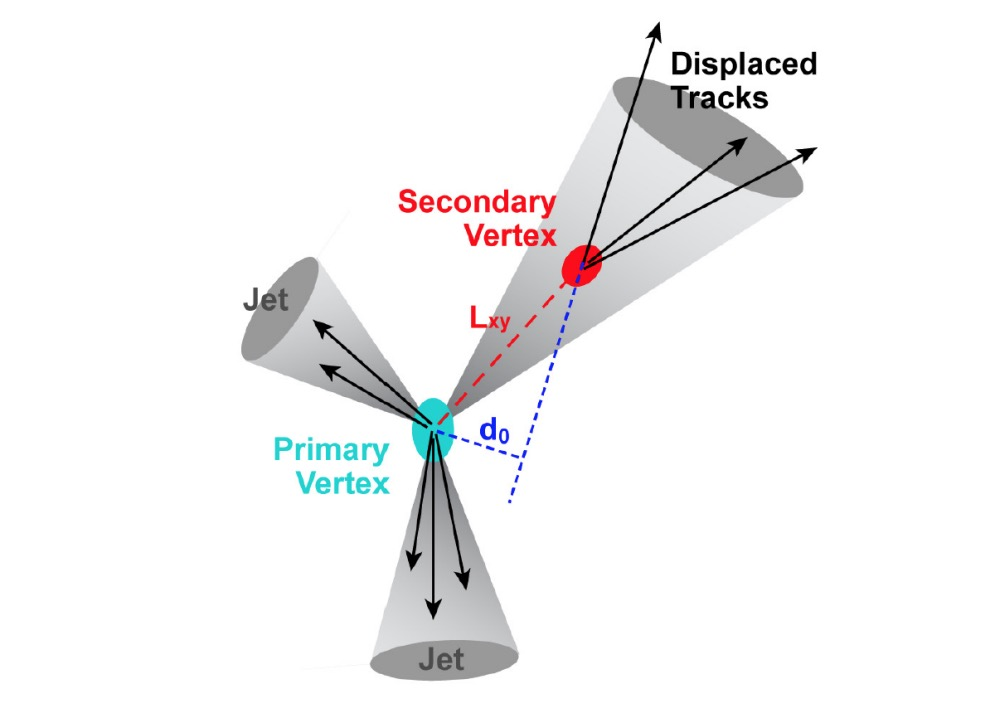
\includegraphics[width=0.75\textwidth]{figuresEXP/ATLASBJET1.jpg}
  \end{center}
  \caption{
包含第二顶点的b-jet示意图。
  }
    \label{fig:ATLASBJET1}
\end{figure}


ATLAS合作组常用的两种机器学习算法是提升决策树和神经网络,这两种机器学习算法在后续章节~\ref{cha:ML}~有简要介绍。
合并上述低级算法的输出并用提升决策树训练出来的b-jet标定算法是MV2~\cite{IPTD}。
而用神经网络构建出来的b-jet标定算法是DL1~\cite{IPTD}。
近年来,实现了一种新的利用递归神经网络发掘b强子衰变径迹之间的空间和运动学关联性的低级算法\textsc{RNNIP}算法~\cite{RNNIP},
DL1r算法~\cite{DLOR1,DLOR2}便是合并了这四种低级算法的输出用神经网络发展出来的新的b-jet标定算法,由于性能比较好,这也是合作组内部推荐的味标定算法,
也是章节~\ref{cha:Dijet}~中物理分析味标定和章节~\ref{cha:Xbb}~中新算法开发所使用的算法。
章节~\ref{cha:Xbb}~中新算法与各种算法性能的对比便是用到上述MV2和DL1r两种算法。
另外,b-jet中b强子半轻子衰变产生的$\mu$子对于b-jet的重建也有一定帮助,
算法SMTnn(Soft muon tagger neural network)便是基于来自重味强子比如b强子或者c强子衰变的$\mu$子的重建而发展出来的一种低级算法,
结合上述五种低级算法的输出用神经网络训练出来的另一种高级算法称为DL1rmu算法。
基于神经网络的高级算法的输出值有三个$p_b$、$p_c$和$p_u$,分别代表jet被判定为b-jet、c-jet或者除前两者之外的light-jet的概率,
其中b-jet作为信号进行训练,另外两种jet作为本底。

\subsection{轻子和光子的重建}
\label{sec:LEPTON}

电子、光子、$\mu$子和$\tau$子的重建都要依赖内部探测器中重建出来的径迹。
电子的重建是通过内部探测器中单个径迹与电磁量能器中的拓扑集群之间的匹配完成的~\cite{LEPTON1,LEPTON2,LEPTON3}。
对于光子,因为一部分高能光子会在内部探测器中转化成正负电子对从而留下径迹,
因此光子的重建是通过内部两条转化径迹与电磁量能器中的拓扑集群之间的匹配或者
无匹配径迹的电磁量能器中单个拓扑集群来实现的~\cite{LEPTON2,LEPTON3}。
除了径迹与拓扑集群之间的匹配要求,为了进一步抑制本底,
还要求电磁辐射和跃迁辐射探测器中的的跃迁辐射强度与重建出来的电子和光子预期表现一致。

$\mu$子是通过内部探测器中径迹与$\mu$子谱仪中径迹之间的匹配来完成的,
而内部探测器接收不到的$\mu$子仅由子谱仪中的径迹来重建~\cite{LEPTON4,LEPTON5}。
$\tau$子产生之后有65\%的概率以强子末态的形式衰变,35\%的概率衰变成更轻的轻子,
由于探测器中来自轻子型衰变$\tau$子的电子和$\mu$子很难与其他过程产生的高能电子和$\mu$子区分开,
因此$\tau$子的重建主要集中在强子型衰变的$\tau$子,它是通过jet重建出来的~\cite{LEPTON6,LEPTON7,LEPTON8}。


\subsection{丢失横动量的重建}
\label{sec:MISSET}

由垂直于束流轴的平面上的动量守恒,末态所有粒子的横动量矢量和应为零,
但由于存在不可探测的粒子比如说标准模型中的中微子,
使得探测器中重建出来的所有末态粒子横动量矢量和不为零,缺失的那部分称为丢失横动量$E_T^{miss}$。
丢失横动量的重建需要利用到ATLAS探测器中所有子探测器重建出来的信息~\cite{LEPTON9},
它的贡献可以分为两部分:
第一部分是硬贡献项(hard term),这部分包含已经重建和校准好的jets和粒子比如电子、光子、$\mu$子和$\tau$子;
第二部分是软贡献项(soft term),这部分由与硬散射顶点关联但不与硬贡献项关联的带电粒子径迹组成,
这样做的目的是为了减小来自堆积事例的影响。
考虑上述两部分贡献,重建出来的$E_T^{miss}$是各个贡献项的矢量和的负数:
\begin{equation} 
\label{eq:MISSET}
\begin{split}
E_T^{miss}=&\underbrace{ -\sum_{electrons} p_T^e -\sum_{photons} p_T^{\gamma}  -\sum_{\tau -leptons} p_T^{\tau_{had}}  -\sum_{muons} p_T^{\mu} }_\text{hard term}
\\
&\underbrace{  -\sum_{unused tracks} p_T^{track} }_\text{soft term}
\end{split}
\end{equation}
















